\documentclass{article}

%% Language and font encodings
\usepackage[english]{babel}
\usepackage[utf8x]{inputenc}
\usepackage[T1]{fontenc}

%% Useful packages
\usepackage{amsmath}
\usepackage{amsfonts}
\usepackage{amssymb}
\usepackage{graphicx}
\usepackage{subcaption}
\usepackage[colorinlistoftodos]{todonotes}
\usepackage[colorlinks=true, allcolors=blue]{hyperref}
\usepackage{showlabels}

\graphicspath{ {figures/} }

% Commands
\newcommand{\alphabet}{\mathcal{A}}
\newcommand{\fullAlignment}{\mathbf{Y}}
\newcommand{\alignmentColumn}{\mathbf{y}}
\newcommand{\alignmentColumnRV}{Y}
\newcommand{\siteSplit}{\tilde{s}}
\newcommand{\siteSplitSet}{\mathcal{S}}
\newcommand{\fullAncestralStates}{\mathbf{H}}
\newcommand{\ancestralStateColumn}{\mathbf{h}}
\newcommand{\ancestralStateColumnRV}{H}
\newcommand{\ancestralSplit}{\tilde{h}}
\newcommand{\ancestralSplitSet}{\mathcal{H}}
\newcommand{\ancestralSplitPartition}{\eta}
\newcommand{\fullAncestralSplitPartitions}{\boldsymbol\eta}

\newcommand{\patternToSplit}{\psi}
\newcommand{\ancestralToSplit}{\xi}

\newcommand{\siteSplitRV}{\Psi}
\newcommand{\ancestralSplitRV}{\Xi}

\newcommand{\nCols}{n}
\newcommand{\nSiteRows}{m}
\newcommand{\nAncestralStateRows}{p}
\newcommand{\nSiteSplits}{q}
\newcommand{\nAncestralSplits}{r}

\newcommand{\shannonDivergence}{D}

\DeclareMathOperator*{\argmax}{argmax}

\allowdisplaybreaks

\title{Possible Inconsistency in Maximum Likelihood Calculation of Ancestral States}
\author{Shaw, Matsen, Minin}

\begin{document}
\maketitle

%comments from Erick:
% >  This is great!
% > - would be great to have all the calculations showing the "refinement" structure written out for the various tree structures (just done by hand and scanned is just fine)
% > - I think of the "refinement" as a partition, so perhaps rather than "empty refinement" we have a "single-element partition"
% > - in order to interpret the site patterns I need to figure out in what order the leaves are labeled
% > - how is ell calculated?
% > - on the numerical sanity check, it doesn't seem clear that the branch lengths can be different than the inferred ones-- they can!
% > - re "general case", agreed though I don't think that we need numerical optimization of branch lengths in a set of a branch length partition-- we can just get the optimal branch length directly. Namely, for each branch, we know all hidden states (given that we are in a set of a partition) and so can count the number of mutations across that branch. From there we have a simple likelihood function, which either has an optimal in the interior or on the boundary of the partition.

\renewcommand{\arraystretch}{1.2} % because otherwise exponents get eaten by \hline


\section*{Introduction}

Classical maximum-likelihood (ML) estimation in phylogenetics operates by integrating out possible ancestral states at the internal nodes of the tree.
Recently, \cite{Sagulenko2017-jo} have suggested using an approximation to ML inference in which the likelihood is maximized jointly across model parameters and ancestral sequences.
This is attractive from a computational perspective: such joint ML inference can proceed according to an iterative procedure in which ML ancestral sequences are first inferred and then model parameters are optimized conditional on the ancestral sequences.
This latter conditional optimization is simpler and more computationally efficient than marginalizing out ancestral sequences and then performing optimization.

Existing consistency proofs for phylogenetics \cite{RoyChoudhury2015-ta} apply only to estimating model parameters when the ancestral sequences have been integrated out of the likelihood.
These proofs do not readily extend to include estimating ancestral states.
Moreover, examples of inconsistency arising from including a large number of additional parameters \cite{Neyman1948-tt} indicate that joint inference of trees and ancestral states may not enjoy good statistical properties.
Although \cite{Sagulenko2017-jo} explicitly warn that their approximation is for the case of branch lengths $\ll 1$ and limit themselves to optimizing branch lengths using this method, this motivates understanding when exactly this approximation breaks down, and what happens when we optimize branch lengths and tree topology using this approximation.

In this paper, we show that the joint inference of trees and ancestral sequences is not consistent in general.
To do so, we use a binary symmetric model and imagine data being generated on the four taxon ``Farris zone'' \cite{Siddall1998-hq} tree, and we construct bounds on the joint likelihood to demarcate a sizeable area of long branch lengths in which joint inference is guaranteed to give the wrong tree in the large-data limit.

\section{Ancestral state reconstruction using maximum likelihood}

We consider the standard phylogenetic likelihood on unrooted phylogenetic trees \cite{Felsenstein2004}.
We assume the character alphabet $\alphabet=\{0,1\}$ and a uniform stationary distribution.
Let $\nSiteRows$ be the number of tips of the tree, and $\nAncestralStateRows = \nSiteRows-2$ the number of internal nodes.
Assume we observe $\nCols$ samples of character data, i.e., an alignment with $\nCols$ columns, $\fullAlignment=[\alignmentColumn_1,\ldots,\alignmentColumn_\nCols]\in\alphabet^{\nSiteRows\times\nCols}$ distributed as the random variable $\alignmentColumnRV$.
The corresponding unobserved ancestral states are $\fullAncestralStates=[\ancestralStateColumn_1,\ldots,\ancestralStateColumn_\nCols]\in\alphabet^{\nAncestralStateRows\times\nCols}$ and distributed as $\ancestralStateColumnRV$.

\subsection{Classical maximum-likelihood inference in phylogenetics}

For a topology $\tau$ and branch lengths $t$, we make the usual assumption of independence between sites, obtaining the likelihood
\begin{equation}
\label{eq:full_likelihood}
%EM given that the H is on the lhs of the conditioning, does it make sense to have it on the rhs of the semicolon? I don't know the convention.
%das: I forgot that standard likelihoods are written with the parameters on the left.
%Since H is like a hidden variable, I went for an expectation-maximization notation, grouping them with the observations.
%It seems a little wonky, though, when we start having maximum likelihood ancestral states depending on \tau,t.
%Oh well...
L_\nCols(\tau, t; \fullAlignment,\fullAncestralStates) = \prod_{i=1}^{\nCols} \ P(\alignmentColumnRV=\alignmentColumn_i, \ancestralStateColumnRV=\ancestralStateColumn_i \mid \tau, t).
\end{equation}
% In particular, we are interested in
% $$
% (\hat{\boldsymbol\xi}, \hat{\tau}, \hat{t}) = \argmax_{\boldsymbol\xi, \tau, t} \ L_n(\mathbf{y};\boldsymbol\xi, \tau, t),
% $$
% which we call the maximum likelihood values of the parameters $(\boldsymbol\xi, \tau, t)$.
% Since the number of elements in $\boldsymbol\xi$ grows with that of the observed data $\mathbf{y}$,
The typical approach to estimate the tree $\tau$ and branch lengths $t$ involves marginalizing across all possible ancestral states
\begin{equation}
\label{eq:marginal_likelihood}
\tilde{L}_\nCols(\tau, t; \fullAlignment) = \sum_{\fullAncestralStates\in\alphabet^{\nAncestralStateRows\times\nCols}} \ L_\nCols(\tau, t; \fullAlignment, \fullAncestralStates)
\end{equation}
and maximizing over the topology and branch lengths to obtain
$$
(\hat{\tau}, \hat{t}) = \argmax_{\tau, t} \  \tilde{L}_\nCols(\tau, t; \fullAlignment).
$$
% The values $\hat{\boldsymbol\xi}$ are then calculated conditional on these estimates.
% More likely in practice we fix a topology $\tau$ and use this marginalization approach to compute $(\hat{\boldsymbol\xi}, \hat{t})$.

\subsection{Joint maximization}

An alternative approach is to do away with the marginalization and directly estimate the maximum likelihood parameters from the fully-observed likelihood in \eqref{eq:full_likelihood}.
One can compute the profile likelihood
\begin{equation}
\label{eq:profile_likelihood}
L_\nCols'(\tau, t; \fullAlignment) = \max_{\fullAncestralStates} \ L_\nCols(\tau, t; \fullAlignment, \fullAncestralStates),
\end{equation}
then estimate the topology and branch lengths via
\begin{equation}
\label{eq:profile_likelihood_topology_bl}
(\hat{\tau}, \hat{t}) = \argmax_{\tau, t} \ L_\nCols'(\tau, t; \fullAlignment),
\end{equation}
using $\hat{\fullAncestralStates}$ maximizing \eqref{eq:profile_likelihood} as an estimate for $\fullAncestralStates$.
Since $\alphabet$ is a discrete set, there exists a maximum \eqref{eq:profile_likelihood}, and \eqref{eq:profile_likelihood_topology_bl} recovers the joint ML values of the unknown parameters.
In general, the functional form of \eqref{eq:profile_likelihood} is determined by inequalities that depend on the unknown $(\tau,t)$.
For this reason, in practice the joint ML strategy estimates $\hat{\fullAncestralStates}$ for a fixed $(\tau,t)$, then $(\hat{\tau},\hat{t})$ given $\hat{\fullAncestralStates}$, maximizing each of these conditional objectives until convergence \cite{Sagulenko2017-jo}.

%EM It seems straightforward to come up with an example of where branch length estimation is inconsistent. It seems like any time a state at an internal node is uncertain we will get different branch lengths by fixing it to the ML state.

\subsection{Site split formulation}

Since we have a finite character alphabet, for a given column $i$ there are a finite number of possibilities of assignments of characters to tips $\alignmentColumn_i$ or internal nodes $\ancestralStateColumn_i$; this results in a simplification of likelihood calculation (we follow Section 8.6 of \cite{Semple2003-em}).
Take the tip labels of $\tau$ to be $\{1,\ldots,\nSiteRows\}$.
For likelihood calculation under the binary symmetric model, we describe a given $\alignmentColumn_i$ as a subset of indices $\siteSplit\subseteq\siteSplitSet:=\{1,\ldots,\nSiteRows-1\}$ with equivalent characters, commonly called a ``site split.''
Indeed, we start by including those tip labels in $\siteSplit$ that are assigned a 1 in the $\alignmentColumn_i$.
Then, because the probability of observing a particular collection of binary characters is equivalent to the probability of its complement under the binary symmetric model, we take the complement if needed to exclude label $\nSiteRows$ from $\siteSplit$.

For topology $\tau$, we define an ordered set of internal node labels $\{1,\ldots,\nAncestralStateRows\}$ for $\ancestralStateColumn_i$ and similarly use a subset of characters $\ancestralSplit\subseteq\ancestralSplitSet:=\{1,\ldots,\nAncestralStateRows\}$ to describe a realization of $\ancestralStateColumn_i$.
In this case the entire set of internal nodes must be enumerated: the probability of observing an ancestral state split, conditional on a site split, is not invariant to taking its complement.

We enumerate the site splits $\siteSplit_j$ of which there are $\nSiteSplits=|\mathcal{P}(\siteSplitSet)|$ in total where $\mathcal{P}$ denotes the power set.
Similarly we enumerate ancestral splits $\ancestralSplit_k$ of which there are $\nAncestralSplits=|\mathcal{P}(\ancestralSplitSet)|$ in total.

This split formulation defines mappings from patterns to splits as
 $$
 \patternToSplit:\alphabet^\nSiteRows\rightarrow\mathcal{P}(\siteSplitSet).
 $$
Given a site pattern--valued random variable $\alignmentColumnRV$, define the random variable
$$
\siteSplitRV := \patternToSplit(\alignmentColumnRV)
$$
that takes corresponding realizations $\siteSplit_j$ for some $j$.

For the $i$th factor of \eqref{eq:full_likelihood},
$$
P(\alignmentColumnRV=\alignmentColumn_i, \ancestralStateColumnRV=\ancestralStateColumn_i \mid \tau, t) = P(\alignmentColumnRV=\alignmentColumn_i \mid \tau, t) \cdot P(\ancestralStateColumnRV=\ancestralStateColumn_i \mid \alignmentColumnRV=\alignmentColumn_i, \tau, t).
$$
As a consequence of assuming a binary symmetric model, taking complements yields
\begin{align*}
    2\cdot P(\alignmentColumnRV=\alignmentColumn_i \mid \tau, t) &= P(\siteSplitRV=\patternToSplit(\alignmentColumn_i) \mid \tau, t) \\
                                                                 &= P(\siteSplitRV=\siteSplit_j \mid \tau, t)
\end{align*}
for some $j$.
For the other term, we define
$$
\ancestralToSplit:\alphabet^\nAncestralStateRows\times\alphabet^\nSiteRows\rightarrow\mathcal{P}(\ancestralSplitSet)
$$
as a mapping of ancestral states and tip states to ancestral state splits.
It is defined by if the tip states have their complements taken or not: if a set of tip labels $\alignmentColumn$ is not contained in $\siteSplitSet$ and thus we must take a complement to become a site split, we let $\ancestralToSplit(\alignmentColumn, \ancestralStateColumn)$ be the complement of $\ancestralStateColumn$; otherwise it is simply $\ancestralStateColumn$.
Note $\ancestralToSplit(\alignmentColumn_i, \cdot)$ is surjective for each $\alignmentColumn_i$.
We define
$$
\ancestralSplitRV := \ancestralToSplit(\alignmentColumnRV, \ancestralStateColumnRV)
$$
for a tip state--valued random variable $\alignmentColumnRV$ and an ancestral state--valued random variable $\ancestralStateColumnRV$.
By considering the case requiring complementing and that not requiring complementing separately,
\begin{align*}
    P(\ancestralStateColumnRV=\ancestralStateColumn_i \mid \alignmentColumnRV=\alignmentColumn_i, \tau, t) &= P(\ancestralSplitRV=\ancestralToSplit(\alignmentColumn_i, \ancestralStateColumn_i) \mid \siteSplitRV=\patternToSplit(\alignmentColumn_i), \tau, t).
\end{align*}
Given $(\tau, t)$, there exists an ordered list of sets $\fullAncestralSplitPartitions(\tau, t)=(\ancestralSplitPartition_1(\tau, t),\ldots,\ancestralSplitPartition_\nSiteSplits(\tau, t))$ such that any element $\xi_j$ of the $j$th component $\ancestralSplitPartition_j(\tau, t)$ satisfies
\begin{align*}
\max_{\ancestralSplit_k\in\mathcal{P}(\ancestralSplitSet)} \ P(\ancestralSplitRV=\ancestralSplit_k \mid \siteSplitRV=\siteSplit_j, \tau, t) &= P(\ancestralSplitRV = \xi_j \mid \siteSplitRV=\siteSplit_j, \tau, t).
\end{align*}
By the surjectivity of $\ancestralToSplit(\alignmentColumn_i, \cdot)$, we also have
\begin{align*}
\max_{\ancestralStateColumn_i} P(\ancestralSplitRV=\ancestralToSplit(\alignmentColumn_i, \ancestralStateColumn_i) \mid \siteSplitRV=\patternToSplit(\alignmentColumn_i), \tau, t) &= P(\ancestralSplitRV = \xi_j \mid \siteSplitRV=\siteSplit_j, \tau, t).
\end{align*}

Let $\xi_j$ be such a choice for each $1 \leq j \leq q$ in the following.
Then, the likelihood in \eqref{eq:profile_likelihood} written as a product over site patterns as opposed to sites is
\begin{align}
L_\nCols'(\tau, t; \fullAlignment) &= \max_{\fullAncestralStates} \ L_\nCols(\tau, t; \fullAlignment, \fullAncestralStates) \nonumber \\
                             &= \prod_{i=1}^{\nCols} \ \max_{\ancestralStateColumn_i} \ P(\alignmentColumnRV=\alignmentColumn_i, \ancestralStateColumnRV=\ancestralStateColumn_i \mid \tau, t) \nonumber \\
                             &\propto \prod_{i=1}^{\nCols} \ \max_{\ancestralStateColumn_i} \ P(\siteSplitRV=\patternToSplit(\alignmentColumn_i) \mid \tau, t) \cdot P(\ancestralSplitRV=\ancestralToSplit(\alignmentColumn_i, \ancestralStateColumn_i) \mid \siteSplitRV=\patternToSplit(\alignmentColumn_i), \tau, t) \nonumber \\
                             &= \prod_{i=1}^{\nCols} \ P(\siteSplitRV=\patternToSplit(\alignmentColumn_i) \mid \tau, t) \cdot \max_{\ancestralStateColumn_i} P(\ancestralSplitRV=\ancestralToSplit(\alignmentColumn_i, \ancestralStateColumn_i) \mid \siteSplitRV=\patternToSplit(\alignmentColumn_i), \tau, t) \nonumber \\
                             &= \prod_{j=1}^{\nSiteSplits} \ \left[P(\siteSplitRV=\siteSplit_j \mid \tau, t)\cdot P(\ancestralSplitRV=\xi_j \mid \siteSplitRV=\siteSplit_j, \tau, t)\right] ^{\nCols_j(\fullAlignment)} \label{eq:site_pattern_likelihood}
\end{align}
where $\nCols_j(\fullAlignment)$ is the number of columns in $\fullAlignment$ where the site split $\siteSplit_j$ or its complement appears.

\paragraph{Example}
\begin{figure}
    \centering
    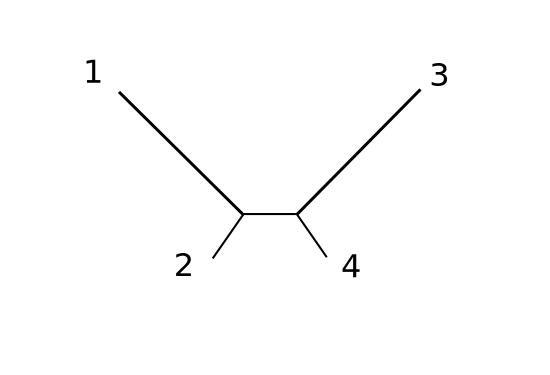
\includegraphics[width=.45\textwidth]{unrooted_four_taxa}
    \caption{Four taxon tree}
\label{fig:four-taxa-tree}
\end{figure}

Consider the fixed, binary four-tip tree $\tau$ in Fig.~\ref{fig:four-taxa-tree}.
The set of all possible character assignments is
\begin{align*}
\mathcal{P}(\{1,2,3,4\}) &= \{\emptyset, \{1,2,3,4\}, \{1\}, \{2,3,4\}, \{2\}, \{1,3,4\}, \{3\}, \{1,2,4\}, \\
                         &\qquad \{1,2\}, \{3,4\}, \{1,3\}, \{2,4\}, \{2,3\}, \{1,4\}, \{1,2,3\}, \{1,4\}\}.
\end{align*}
where each set indicates the tips assigned the character $1$.
For example, $\emptyset$ is the labeling $0000$ and $\{1,3,4\}$ is the labeling $1011$.
Symmetry allows us to group adjacent pairs in $\mathcal{P}(\{1,2,3,4\})$ into equiprobable splits, letting $\siteSplitSet=\{1,2,3\}$.
The unique site splits, collapsing complements, are
\begin{align*}
    \mathcal{P}(\siteSplitSet) &= \{\emptyset, \{1\}, \{2\}, \{3\}, \{1,2\}, \{1,3\}, \{2,3\}, \{1,2,3\}\} \\
& := \{\siteSplit_1, \ldots, \siteSplit_8\}.
\end{align*}
Since we identify character complements, we do not consider the additional splits
$$
\mathcal{P}(\{1,2,3,4\}) \setminus \mathcal{P}(\siteSplitSet) = \{\{1,2,3,4\}, \{2,3,4\}, \{1,3,4\}, \{1,2,4\}, \{3,4\}, \{2,4\}, \{1,4\}, \{4\}\},
$$
the symmetry of the binary character model allowing us to focus only on the elements of $\mathcal{P}(\siteSplitSet)$.
This tree has two internal nodes with $\ancestralSplitSet=\{1,2\}$ and unique ancestral state splits
$$
\mathcal{P}(\ancestralSplitSet) = \{\emptyset, \{1\}, \{2\}, \{1,2\}\}.
$$
Internal node $\{1\}$ is the node connected to leaves $\{1\}$ and $\{2\}$ and internal node $\{2\}$ connected to leaves $\{3\}$ and $\{4\}$.
The mapping from characters to splits in this case will depend on the characters at the tips and the ancestral states.
For example, we take both $\patternToSplit(0000)=\emptyset$ and $\patternToSplit(1111)=\emptyset$.
Similarly, we have $\ancestralToSplit(0000, 00) = \emptyset$ and $\ancestralToSplit(1111, 11)=\emptyset$, needing to take the complement of all the characters present on the tree to identify splits.
We cannot identify complements for ancestral states since, for $\siteSplit\in\mathcal{P}(\siteSplitSet)$,
$$
P(\ancestralSplitRV=\emptyset \mid \siteSplitRV=\siteSplit, \tau, t)\neq P(\ancestralSplitRV=\{1,2\} \mid \siteSplitRV=\siteSplit, \tau, t)
$$
in general.

For each site split $\siteSplit\in\mathcal{P}(\siteSplitSet)$, we maximize the likelihood over all $\ancestralSplit\in\mathcal{P}(\ancestralSplitSet)$.
A maximum occurs at one of possibly several ancestral splits in $\mathcal{P}(\ancestralSplitSet)$; for the $j$th site split, define $\ancestralSplitPartition_j(\tau, t)\subset\mathcal{P}(\ancestralSplitSet)$ as the set of most likely ancestral splits for that particular site split, topology and set of branch lengths.
As a simple example, say all branch lengths correspond to a probability $p$ ($< 1/2$) of changing character along that branch.
The probabilities of observing ancestral splits for $\siteSplit_1=\emptyset$ are
$$
P(\ancestralSplitRV=\emptyset \mid \siteSplitRV=\emptyset, \tau, t) =
(1-p)^5,
$$
$$
P(\ancestralSplitRV=\{1\} \mid \siteSplitRV=\emptyset, \tau, t) =
P(\ancestralSplitRV=\{2\} \mid \siteSplitRV=\emptyset, \tau, t) =
p^3(1-p)^2,
$$
$$
P(\ancestralSplitRV=\{1,2\} \mid \siteSplitRV=\emptyset, \tau, t) =
p^4(1-p).
$$
The set of most likely ancestral states contains a single element, here $\ancestralSplitPartition_1(\tau, p)=\{\emptyset\}$.
Then, taking $\xi_1\in\ancestralSplitPartition_1(\tau, p)$ we have
$$
P(\ancestralSplitRV=\xi_1 \mid \siteSplitRV=\emptyset, \tau, t) =
(1-p)^5.
$$
For $\siteSplit_6=\{1,3\}$ we have
$$
P(\ancestralSplitRV=\emptyset \mid \siteSplitRV=\{1,3\}, \tau, t) =
P(\ancestralSplitRV=\{1,2\} \mid \siteSplitRV=\{1,3\}, \tau, t) =
p^2(1-p)^3,
$$
$$
P(\ancestralSplitRV=\{1\} \mid \siteSplitRV=\{1,3\}, \tau, t) =
P(\ancestralSplitRV=\{2\} \mid \siteSplitRV=\{1,3\}, \tau, t) =
p^3(1-p)^2.
$$
Here, the set of most likely ancestral states is $\ancestralSplitPartition_6(\tau, p)=\{\emptyset,\{1,2\}\}$, and, for $\xi_6\in\ancestralSplitPartition_6(\tau, p)$,
$$
P(\ancestralSplitRV=\xi_6 \mid \siteSplitRV=\{1,3\}, \tau, t) =
p^2(1-p)^3.
$$

\subsection{Showing inconsistency}

We are interested in the properties of the objective function being maximized in \eqref{eq:site_pattern_likelihood} as data becomes plentiful.
Let
$$
L_\nCols''(\tau, t; \fullAlignment, \fullAncestralSplitPartitions(\tau, t)) = \prod_{j=1}^{\nSiteSplits} \ \left[P(\siteSplitRV=\siteSplit_j \mid \tau, t) \cdot P(\ancestralSplitRV=\xi_j \mid \siteSplitRV=\siteSplit_j, \tau, t)\right] ^{\nCols_j(\fullAlignment)}
$$
be the final product in \eqref{eq:site_pattern_likelihood}.
Assume our $\nCols$ observations were generated from a model with parameters $(\tau^*, t^*)$.
We have
\begin{align}
    \frac{1}{\nCols} \log L_\nCols''(\tau, t; \fullAlignment, \fullAncestralSplitPartitions(\tau,t))
        &= \sum_{j=1}^\nSiteSplits \frac{\nCols_j(\fullAlignment)}{\nCols}\cdot  \log P(\siteSplitRV=\siteSplit_j, \ancestralSplitRV=\xi_j \mid \tau, t) \\
        &= \sum_{j=1}^\nSiteSplits \frac{\nCols_j(\fullAlignment)}{\nCols}\cdot [\log P(\siteSplitRV=\siteSplit_j \mid \tau, t) +
            \log P(\ancestralSplitRV=\xi_j \mid \siteSplitRV=\siteSplit_j , \tau, t)]
\end{align}
so that, in the limit of infinite data,
\begin{equation}
    \frac{1}{\nCols} \log L_\nCols''(\tau, t; \fullAlignment, \fullAncestralSplitPartitions(\tau, t)) \rightarrow \sum_{j=1}^\nSiteSplits P(\siteSplitRV=\siteSplit_j \mid \tau^*, t^*) \cdot [\log P(\siteSplitRV=\siteSplit_j \mid \tau, t) + \log P(\ancestralSplitRV=\xi_j \mid \siteSplitRV=\siteSplit_j , \tau, t)]. \label{eq:site_pattern_profile_likelihood_mean}
\end{equation}
Define the divergence quantity
$$
\shannonDivergence_{\tau^*,t^*}(\tau,t) = \sum_{j=1}^\nSiteSplits P(\siteSplitRV=\siteSplit_j \mid \tau^*, t^*)\cdot\log P(\siteSplitRV=\siteSplit_j \mid \tau, t),
$$
and the partial log likelihood
$$
\tilde{\ell}_{\tau^*,t^*}(\tau, t; \fullAncestralSplitPartitions(\tau,t)) = \sum_{j=1}^\nSiteSplits P(\siteSplitRV=\siteSplit_j \mid \tau^*, t^*)\cdot\log P(\ancestralSplitRV=\xi_j \mid \siteSplitRV = \siteSplit_j, \tau, t)
$$
so that \eqref{eq:site_pattern_profile_likelihood_mean} becomes
\begin{equation}
    \label{eq:log_likelihood_simplified}
    \ell_{\tau^*,t^*}(\tau, t; \fullAncestralSplitPartitions(\tau,t)) = \shannonDivergence_{\tau^*,t^*}(\tau,t) + \tilde{\ell}_{\tau^*,t^*}(\tau, t; \fullAncestralSplitPartitions(\tau,t)).
\end{equation}
For data generated from $(\tau^*, t^*)$, we have an inconsistency if
\begin{equation}
\label{eq:inconsistency_inequality}
\ell_{\tau^*,t^*}(\tau', \hat{t}_1; \fullAncestralSplitPartitions(\tau', \hat{t}_1)) > \ell_{\tau^*,t^*}(\tau^*, \hat{t}_2; \fullAncestralSplitPartitions(\tau^*, \hat{t}_2))
\end{equation}
for $\tau'\neq\tau^*$ with $\{\hat{t}_1,\fullAncestralSplitPartitions(\tau', \hat{t}_1)\}$ and $\{\hat{t}_2,\fullAncestralSplitPartitions(\tau^*, \hat{t}_2)\}$ estimated by maximizing $\tilde{\ell}_{\tau^*,t^*}$ with respect to the branch lengths and the internal states for $\tau = \tau'$ and $\tau^*$, respectively.
By Gibbs' inequality, $\shannonDivergence_{\tau^*,t^*}(\tau,t)$ is maximized when $(\tau,t) = (\tau^*,t^*)$, so any example of inconsistency must overcome that difference with substantially greater partial likelihoods on the non-generating topology.
In the next section, we show that such examples exist.

\section{Inconsistency of joint maximum likelihood}

\subsection{Bounding the likelihoods}

Our approach seeks bounds for the terms inside the maximization in \eqref{eq:log_likelihood_simplified}.
We obtain
%EM Does it really make sense to talk about taking the max over \fullAncestralSplitPartitions(\tau,t)? This is already defined. I suggest just taking the max over \fullAncestralSplitPartitions as a variable.
$$
\max_{t} \ \ell_{\tau^*,t^*}(\tau, t; \fullAncestralSplitPartitions(\tau,t)) \le
    \shannonDivergence_{\tau^*,t^*}(\tau^*,t^*)
    + \tilde{\ell}_{\tau^*,t^*}(\tau, \hat{t}; \fullAncestralSplitPartitions(\tau, \hat{t}))
$$
as an upper bound for the joint maximum of \eqref{eq:log_likelihood_simplified} using Gibbs's inequality
$$
\shannonDivergence_{\tau^*,t^*}(\tau,t) \le \shannonDivergence_{\tau^*,t^*}(\tau^*,t^*)
$$
and
$$
\hat{t} = \argmax_{t} \ \tilde{\ell}_{\tau^*,t^*}(\tau, t; \fullAncestralSplitPartitions(\tau,t)).
$$
Similarly, we have the lower bound
$$
\max_{t} \ \ell_{\tau^*,t^*}(\tau, t; \fullAncestralSplitPartitions(\tau,t)) \ge
    \shannonDivergence_{\tau^*,t^*}(\tau,\hat{t})
    + \tilde{\ell}_{\tau^*,t^*}(\tau, \hat{t}; \fullAncestralSplitPartitions(\tau, \hat{t})).
$$

\subsection{Parameter setting}

\begin{figure}
\centering
\begin{subfigure}{.45\linewidth}
\centering
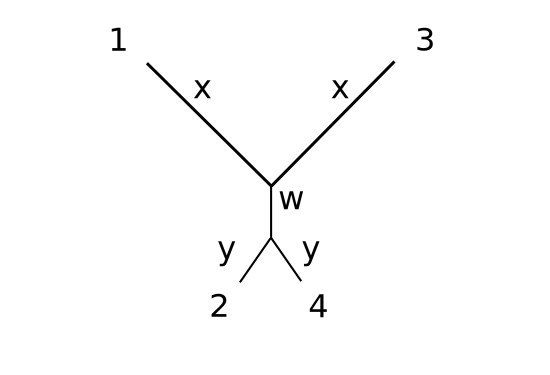
\includegraphics[width=.95\textwidth]{farris_blank}
\caption[short]{Farris topology $\tau_1$}
\end{subfigure}
\begin{subfigure}{.45\linewidth}
\centering
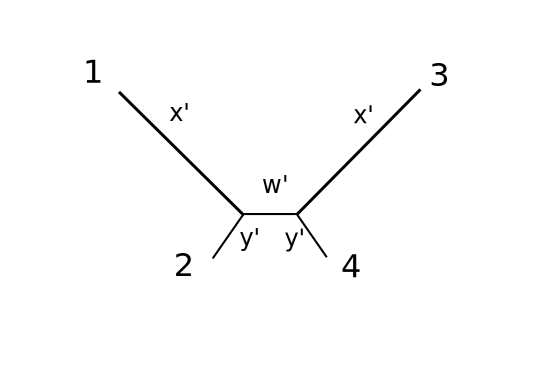
\includegraphics[width=.95\textwidth]{felsenstein_blank}
\caption[short]{Felsenstein topology $\tau_2$}
\end{subfigure}
\caption{Two simple topologies}
\label{fig:farris-fels-top}
\end{figure}

Define the Farris topology $\tau_1$ and the Felsenstein topology $\tau_2$ as in Figure~\ref{fig:farris-fels-top}.
We parameterize the branches of these trees \textbf{not with the standard notion of branch length in terms of number of substitutions per site}, but with a parameter such that the probability of a substitution on a branch with parameter $\theta$ is $p_\theta = (1-\theta)/2$ while the probability of no substitution is $(1+\theta)/2$.
This parametrization has been called edge ``fidelity'' as it quantifies the fidelity of transmission of the ancestral state along an edge \cite{Matsen2007-jq}.
Fidelities have useful algebraic properties, such as the ability to write generating probabilities using the Hadamard transform.

Let $\{x',y',w'\}\in[0,1]^3$ be three fidelities and $\{p_x',p_y',p_w'\}\in[0,1/2]^3$ the corresponding substitution probabilities.
Call $t=\{x',y',w'\}$ and $t^*=\{x,y,y\}$, i.e., $t^*$ constrains the bottom three branches to share the same parameter, the classical construction of this topology.

We now show that, in the case of the Farris tree topology, fixing both the top two branch lengths to be equal and the bottom two branch lengths to be equal does not change the value of the likelihood.
Consider the Farris topology with arbitrary branch lengths, i.e., $\tilde{t}=\{x_1,y_1,x_2,y_2,w\}$ with edge ordering in the order of the taxa, then the internal branch last.
%EM complete to introduce: We now note that exchanging $x_1$ and $x_2$, or $y_1$ or $y_2$, does not change ...
%EM please be a little more specific than just $ell$, because there are lots of variants-- e.g. likelihood with what data?
Using the Hadamard transform approach outlined in 8.6 of Semple and Steel \cite{Semple2003-em}, we calculate the generating probabilities on the Farris tree topology.
For site split $\emptyset$,
\begin{align*}
    P(\siteSplitRV=\emptyset\mid \tau_1, \tilde{t}) & = \frac{1}{8} (1 + x_1x_2 +  y_1y_2 +  x_1y_1w + x_1y_2w + y_1x_2w + x_2y_2w + x_1y_1x_2y_2) \\
                                              & = \frac{1}{8} (1 + x_1x_2 +  y_1y_2 +  w[x_1y_1 + x_1y_2 + y_1x_2 + x_2y_2] + x_1y_1x_2y_2) \\
                                              & = \frac{1}{8} (1 + x_1x_2 +  y_1y_2 +  w[x_1 + x_2][y_1 + y_2] + x_1y_1x_2y_2).
\end{align*}
and this probability is unchanged when $x_1$ is exchanged with $x_2$ and $y_1$ is exchanged with $y_2$.
All other generating probabilities will differ only in the signs of each term.
For example, for site split $\{1\}$ we have
\begin{align*}
    P(\siteSplitRV=\{1\}\mid \tau_1, \tilde{t}) & = \frac{1}{8} (1 - x_1x_2 +  y_1y_2 +  w[-x_1 + x_2][y_1 + y_2] - x_1y_1x_2y_2)
\end{align*}
and for site split $\{3\}$ we have
\begin{align*}
    P(\siteSplitRV=\{3\}\mid \tau_1, \tilde{t}) & = \frac{1}{8} (1 - x_1x_2 +  y_1y_2 +  w[x_1 - x_2][y_1 + y_2] - x_1y_1x_2y_2)
\end{align*}
meaning if we exchange the values of $x_1$ and $x_2$ then these probabilities swap values.
The corresponding possibilities for the likelihood values are
\begin{align*}
    P(\ancestralSplitRV=\emptyset \mid \siteSplitRV=\{1\}, \tau_1, \tilde{t}) &= \frac{1}{32}(1-x_1)(1+x_2)(1+w)(1+y_1)(1+y_2); \\
    P(\ancestralSplitRV=\{1\} \mid \siteSplitRV=\{1\}, \tau_1, \tilde{t}) &= \frac{1}{32}(1+x_1)(1-x_2)(1-w)(1+y_1)(1+y_2); \\
    P(\ancestralSplitRV=\{2\} \mid \siteSplitRV=\{1\}, \tau_1, \tilde{t}) &= \frac{1}{32}(1-x_1)(1+x_2)(1-w)(1-y_1)(1-y_2); \\
    P(\ancestralSplitRV=\{1,2\} \mid \siteSplitRV=\{1\}, \tau_1, \tilde{t}) &= \frac{1}{32}(1+x_1)(1-x_2)(1+w)(1-y_1)(1-y_2);
\end{align*}
for site split $\{1\}$ and
\begin{align*}
        P(\ancestralSplitRV=\emptyset \mid \siteSplitRV=\{3\}, \tau_1, \tilde{t}) &= \frac{1}{32}(1+x_1)(1-x_2)(1+w)(1+y_1)(1+y_2); \\
    P(\ancestralSplitRV=\{1\} \mid \siteSplitRV=\{3\}, \tau_1, \tilde{t}) &= \frac{1}{32}(1-x_1)(1+x_2)(1-w)(1+y_1)(1+y_2); \\
    P(\ancestralSplitRV=\{2\} \mid \siteSplitRV=\{3\}, \tau_1, \tilde{t}) &= \frac{1}{32}(1+x_1)(1-x_2)(1-w)(1-y_1)(1-y_2); \\
    P(\ancestralSplitRV=\{1,2\} \mid \siteSplitRV=\{3\}, \tau_1, \tilde{t}) &= \frac{1}{32}(1-x_1)(1+x_2)(1+w)(1-y_1)(1-y_2);
\end{align*}
for site split $\{3\}$, which also both swap values when $x_1$ and $x_2$ are exchanged.

The same can be done for the splits $\{2\}$ and $\{1,2,3\}$ by exchanging $y_1$ and $y_2$ as well as $\{1,2\}$ and $\{1,3\}$ by exchanging both $x_1$ with $x_2$ and $y_1$ with $y_2$.
The split $\{1,3\}$ is unchanged by exchanging $x_1$ with $x_2$ and $y_1$ with $y_2$.

In summary, exchanging $x_1$ and $x_2$ does not change the value of the log likelihood $\ell_{\tau_1,t^*}(\tau_1, \tilde{t}; \fullAncestralSplitPartitions(\tau_1,\tilde{t}))$, and thus $x_1=x_2$ at the maximum.
The analogous statement holds for $y_1$ and $y_2$.
The Felsenstein topology does not admit this property, but, since we are interested in a lower bound for this topology, we simplify the objective function by constraining $x_1=x_2$ and $y_1=y_2$ similarly.

Table~\ref{tab:sitepatprob} contains calculations of site pattern frequencies under these two topologies.
Table~\ref{tab:likelihoods} contains calculations of likelihood values for fixed site patterns and topologies that have been maximized over ancestral state patterns.
Tables~\ref{tab:farris_likelihoods} and~\ref{tab:fels_likelihoods} contain the values of the likelihood for all possible ancestral states.

\begin{table}
\centering
\begin{tabular}{|l|l|l|}
    \hline
$\siteSplit_j$   &$P(\siteSplitRV=\siteSplit_j \mid \tau_1,t)$&$P(\siteSplitRV=\siteSplit_j \mid \tau_2,t)$\\
    \hline
    $\emptyset$    &$1+x'^2+y'^2+4x'y'w'+x'^2y'^2$&$1+2x'y'+2x'y'w'+x'^2w'+y'^2w'+x'^2y'^2$\\
    $\{1\}$        &$1-x'^2+y'^2-x'^2y'^2$&$1-x'^2w'+y'^2w'-x'^2y'^2$\\
    $\{2\}$        &$1+x'^2-y'^2-x'^2y'^2$&$1+x'^2w'-y'^2w'-x'^2y'^2$\\
    $\{3\}$        &$1-x'^2+y'^2-x'^2y'^2$&$1-x'^2w'+y'^2w'-x'^2y'^2$\\
    $\{1,2\}$      &$1-x'^2-y'^2+x'^2y'^2$&$1+2x'y'-2x'y'w'-x'^2w'-y'^2w'+x'^2y'^2$\\
    $\{1,3\}$      &$1+x'^2+y'^2-4x'y'w'+x'^2y'^2$&$1-2x'y'-2x'y'w'+x'^2w'+y'^2w'+x'^2y'^2$\\
    $\{2,3\}$      &$1-x'^2-y'^2+x'^2y'^2$&$1-2x'y'+2x'y'w'-x'^2w'-y'^2w'+x'^2y'^2$\\
    $\{1,2,3\}$    &$1+x'^2-y'^2-x'^2y'^2$&$1+x'^2w'-y'^2w'-x'^2y'^2$\\
    \hline
\end{tabular}
\caption{Site pattern probabilities.
All values are multiplied by $1/8$.}
\label{tab:sitepatprob}
\end{table}

\begin{table}
\centering
\begin{tabular}{|l|ll|}
    \multicolumn{3}{c}{$\tau=\tau_1$}\\
    \hline
    $\siteSplit_j$    & $\ancestralSplitPartition_j(\tau, t)$ & $P(\ancestralSplitRV=\xi_j \mid \siteSplitRV=\siteSplit_j,\tau,t)$\\
    \hline
    $\emptyset$&
    $\emptyset$&
    $(1+x')^2   (1+w')(1+y')^2$\\
     $\{1\}$    &
    $\emptyset$&
    $(1+x')(1-x')(1+w')(1+y')^2$\\
     $\{2\}$    &
    $\emptyset$&
    $(1+x')^2   (1+w')(1+y')(1-y')$\\
     $\{3\}$    &
    $\emptyset$&
    $(1+x')(1-x')(1+w')(1+y')^2$\\
    $\{1,2\}$  &
    $\{\emptyset,\{1,2\}\}$&
    $(1+x')(1-x')(1+w')(1+y')(1-y')$\\
    $\{1,3\}$  &
    $\left\{\begin{array}{l}
                    \emptyset\\
                    %EM Shouldn't this be \{1\}\\ ? Or perhaps the ordering of internal nodes is not what I thought?
                    \{1\}\\
                    \{1,2\}
                \end{array}\right.$&
    $\begin{array}{l}
                    (1-x')^2   (1+w')(1+y')^2\\
                    (1+x')^2   (1-w')(1+y')^2\\
                    (1+x')^2   (1+w')(1-y')^2
                \end{array}$\\
    $\{2,3\}$  &
                $\{\emptyset,\{1,2\}\}$&
                $(1+x')(1-x')(1+w')(1+y')(1-y')$\\
    $\{1,2,3\}$&
                $\{1,2\}$&
                $(1+x')^2   (1+w')(1+y')(1-y')$\\
    \hline
    \multicolumn{3}{c}{$\tau=\tau_2$}\\
    \hline
    $\siteSplit_j$    & $\ancestralSplitPartition_j(\tau, t)$ & $P(\ancestralSplitRV=\xi_j \mid \siteSplitRV=\siteSplit_j,\tau,t)$\\
    \hline
    $\emptyset$       &$\emptyset$&$(1+x')^2   (1+w')(1+y')^2$\\
    $\{1\}$          &
    $\left\{\begin{array}{l}
                    \emptyset\\
                    \{1\}
                \end{array}\right.$&
    $\begin{array}{l}
                        (1+x')(1-x')(1+w')(1+y')^2\\
                        (1+x')^2   (1-w')(1+y')(1-y')
                    \end{array}$\\
      $\{2\}$          &
    $\left\{\begin{array}{l}
                    \emptyset\\
                    \{1\}
                \end{array}\right.$&
    $\begin{array}{l}
                    (1+x')^2   (1+w')(1+y')(1-y')\\
                    (1+x')(1-x')(1-w')(1+y')^2
                    \end{array}$\\
      $\{3\}$          &
    $\left\{\begin{array}{l}
                    \emptyset\\
                    \{2\}
                \end{array}\right.$&
    $\begin{array}{l}
                    (1+x')(1-x')(1+w')(1+y')^2\\
                    (1+x')^2   (1-w')(1+y')(1-y')
                    \end{array}$\\
     $\{1,2\}$         &
    $\left\{\begin{array}{l}
                    \{\emptyset,\{1,2\}\}\\
                    \{1\}
                \end{array}\right.$&
    $\begin{array}{l}
                    (1+x')(1-x')(1+w')(1+y')(1-y')\\
                    (1+x')^2   (1-w')(1+y')^2
                    \end{array}$\\
     $\{1,3\}$         &
    $\left\{\begin{array}{l}
                    \emptyset\\
                    \{\{1\},\{2\}\}\\
                    \{1,2\}
                \end{array}\right.$&
    $\begin{array}{l}
                    (1-x')^2   (1+w')(1+y')^2\\
                    (1+x')(1-x')(1-w')(1+y')(1-y')\\
                    (1+x')^2   (1+w')(1-y')^2
                    \end{array}$\\
      $\{2,3\}$        &
    $\left\{\begin{array}{l}
                    \{\emptyset,\{1,2\}\}\\
                    \{1\}\\
                    \{2\}
                \end{array}\right.$&
    $\begin{array}{l}
                    (1+x')(1-x')(1+w')(1+y')(1-y')\\
                    (1-x')^2   (1-w')(1+y')^2\\
                    (1+x')^2   (1-w')(1-y')^2
                    \end{array}$\\
     $\{1,2,3\}$       &
    $\left\{\begin{array}{l}
                    \{2\} \\
                    \{1,2\}
                \end{array}\right.$&
    $\begin{array}{l}
                    (1+x')(1-x')(1-w')(1+y')^2 \\
                    (1+x')^2   (1+w')(1+y')(1-y')
                    \end{array}$\\
    \hline
\end{tabular}
\caption{Likelihood calculations for all site patterns and ancestral state partitions.
All values multiplied by $1/32$.
Likelihoods with multiple entries have maxima determined by unknown branch length parameters.
See Appendix for full calculations.}
\label{tab:likelihoods}
\end{table}

\subsubsection{Upper bound for Farris tree likelihood}

Assume $\tau^*=\tau_1$ and $t^*=\{x,y,y\}$.
For compactness, define
$$
p_{\emptyset} = P(\siteSplitRV=\emptyset \mid \tau=\tau_1,t=\{x,y,y\})
$$
with similar definitions for the remaining generating probabilities.
The full Farris tree log likelihood takes one of three values depending on branch lengths---assume for now the we are only interested in the ancestral state split $\{1\}$ for the site split $\{1,3\}$.
Directly substituting in \eqref{eq:site_pattern_likelihood}, the log likelihood is
\begin{align*}
    \ell_{\tau_1,\{x,y,y\}}(\tau_1, \{x',y',w'\}; \fullAncestralSplitPartitions(\tau_1,\{x',y',w'\}))
    &=        p_{\emptyset}  \cdot\log(1+x'^2+y'^2+4x'y'w'+x'^2y'^2) \\
    &\qquad + p_{1}          \cdot\log(1-x'^2+y'^2-x'^2y'^2) \\
    &\qquad + p_{2}          \cdot\log(1+x'^2-y'^2-x'^2y'^2) \\
    &\qquad + p_{3}          \cdot\log(1-x'^2+y'^2-x'^2y'^2) \\
    &\qquad + p_{12}         \cdot\log(1-x'^2-y'^2+x'^2y'^2) \\
    &\qquad + p_{13}         \cdot\log(1+x'^2+y'^2-4x'y'w'+x'^2y'^2) \\
    &\qquad + p_{23}         \cdot\log(1-x'^2-y'^2+x'^2y'^2) \\
    &\qquad + p_{123}        \cdot\log(1+x'^2-y'^2-x'^2y'^2) \\
    &\qquad + p_{\emptyset}  \cdot\log((1+x')^2   (1+w')(1+y')^2) \\
    &\qquad + p_{1}          \cdot\log((1+x')(1-x')(1+w')(1+y')^2) \\
    &\qquad + p_{2}          \cdot\log((1+x')^2   (1+w')(1+y')(1-y')) \\
    &\qquad + p_{3}          \cdot\log((1+x')(1-x')(1+w')(1+y')^2) \\
    &\qquad + p_{12}         \cdot\log((1+x')(1-x')(1+w')(1+y')(1-y')) \\
    &\qquad + p_{13}         \cdot\log((1+x')^2   (1-w')(1+y')^2) \\
    &\qquad + p_{23}         \cdot\log((1+x')(1-x')(1+w')(1+y')(1-y')) \\
    &\qquad + p_{123}        \cdot\log((1+x')^2   (1+w')(1+y')(1-y')).
\end{align*}
Seeking an upper bound, we use the facts that, for $x',y'\in[0,1]$,
\begin{align*}
(1-x'^2+y'^2-x'^2y'^2) & = (1+x')(1-x')(1+y'^2) \le (1+x')(1-x')(1+y') \\
(1+x'^2-y'^2-x'^2y'^2) & = (1+x'^2)(1+y')(1-y') \le (1+x')(1+y')(1-y') \\
(1+x'^2+y'^2+x'^2y'^2) & = (1+x'^2)(1+y'^2) \le (1+x')(1+y') \\
4x'y' & = 2x' \cdot 2y' \le (1+x'^2)(1+y'^2) \le (1+x')(1+y').
\end{align*}
The term $p_{\emptyset}$ is bounded as
\begin{align*}
    p_{\emptyset} & = \log(1+x'^2+y'^2+4x'y'w'+x'^2y'^2) \\
                  & \le \log(1+x'^2+y'^2+4x'y'+x'^2y'^2) \\
                  & \le \log(2(1+x')(1+y'))
\end{align*}
and $p_{13}$ is bounded as
\begin{align*}
    p_{13} & = \log(1+x'^2+y'^2-4x'y'w'+x'^2y'^2) \\
                  & \le \log(1+x'^2+y'^2+x'^2y'^2) \\
                  & \le \log((1+x')(1+y')).
\end{align*}
Factoring and making these substitutions results in
\begin{align*}
    \ell_{\tau_1,\{x,y,y\}}(\tau_1, \{x',y',w'\}; \fullAncestralSplitPartitions(\tau_1,\{x',y',w'\}))
    &\le      p_{\emptyset}  \cdot\log(2(1+x')(1+y')) \\
    &\qquad + p_{1}          \cdot\log((1+x')(1-x')(1+y')) \\
    &\qquad + p_{2}          \cdot\log((1+x')(1+y')(1-y')) \\
    &\qquad + p_{3}          \cdot\log((1+x')(1-x')(1+y')) \\
    &\qquad + p_{12}         \cdot\log((1+x')(1-x')(1+y')(1-y')) \\
    &\qquad + p_{13}         \cdot\log((1+x')(1+y')) \\
    &\qquad + p_{23}         \cdot\log((1+x')(1-x')(1+y')(1-y')) \\
    &\qquad + p_{123}        \cdot\log((1+x')(1+y')(1-y')) \\
    &\qquad + p_{\emptyset}  \cdot\log((1+x')^2   (1+w')(1+y')^2) \\
    &\qquad + p_{1}          \cdot\log((1+x')(1-x')(1+w')(1+y')^2) \\
    &\qquad + p_{2}          \cdot\log((1+x')^2   (1+w')(1+y')(1-y')) \\
    &\qquad + p_{3}          \cdot\log((1+x')(1-x')(1+w')(1+y')^2) \\
    &\qquad + p_{12}         \cdot\log((1+x')(1-x')(1+w')(1+y')(1-y')) \\
    &\qquad + p_{13}         \cdot\log((1+x')^2   (1-w')(1+y')^2) \\
    &\qquad + p_{23}         \cdot\log((1+x')(1-x')(1+w')(1+y')(1-y')) \\
    &\qquad + p_{123}        \cdot\log((1+x')^2   (1+w')(1+y')(1-y')).
\end{align*}
Grouping together like terms,
\begin{align*}
    \ell_{\tau_1,\{x,y,y\}}(\tau_1, \{x',y',w'\}; \fullAncestralSplitPartitions(\tau_1,\{x',y',w'\}))
%EM Afraid I don't see how all of the p_emptyset terms are bounded above here.
    &\le      p_{\emptyset}  \cdot\log(2) \\
    &\qquad + \log(1+x') \\
    &\qquad + (p_{1}+p_{3}+p_{12}+p_{23})\cdot\log(1-x') \\
    &\qquad + \log(1+y') \\
    &\qquad + (p_{2}+p_{12}+p_{23}+p_{123})\cdot\log(1-y') \\
    &\qquad + (2-p_{1}-p_{3}-p_{12}-p_{23})\cdot\log(1+x') \\
    &\qquad + (p_{1}+p_{3}+p_{12}+p_{23})\cdot\log(1-x') \\
    &\qquad + (2-p_{2}-p_{12}-p_{23}-p_{123})\cdot\log(1+y') \\
    &\qquad + (p_{2}+p_{12}+p_{23}+p_{123})\cdot\log(1-y') \\
    &\qquad + (1-p_{13})\cdot\log(1+w') \\
    &\qquad + p_{13}\cdot\log(1-w'),
\end{align*}
which equals
\begin{align*}
    \ell_{\tau_1,\{x,y,y\}}(\tau_1, \{x',y',w'\}; \fullAncestralSplitPartitions(\tau_1,\{x',y',w'\}))
    &\le      p_{\emptyset}  \cdot\log(2) \\
    &\qquad + (3-p_{1}-p_{3}-p_{12}-p_{23})\cdot\log(1+x') \\
    &\qquad + 2(p_{1}+p_{3}+p_{12}+p_{23})\cdot\log(1-x') \\
    &\qquad + (3-p_{2}-p_{12}-p_{23}-p_{123})\cdot\log(1+y') \\
    &\qquad + 2(p_{2}+p_{12}+p_{23}+p_{123})\cdot\log(1-y') \\
    &\qquad + (1-p_{13})\cdot\log(1+w') \\
    &\qquad + p_{13}\cdot\log(1-w').
\end{align*}
To make matters further compact, let
$$
a_{1} = 3-p_{1}-p_{3}-p_{12}-p_{23},
$$
$$
a_{2} = 2(p_{1}+p_{3}+p_{12}+p_{23}),
$$
$$
a_{3} = 3-p_{2}-p_{12}-p_{23}-p_{123},
$$
$$
a_{4} = 2(p_{2}+p_{12}+p_{23}+p_{123}),
$$
where
\begin{align*}
    \ell_{\tau_1,\{x,y,y\}}(\tau_1, \{x',y',w'\}; \fullAncestralSplitPartitions(\tau_1,\{x',y',w'\}))
    &\le      p_{\emptyset}  \cdot\log(2) \\
    &\qquad + a_{1}\cdot\log(1+x') \\
    &\qquad + a_{2}\cdot\log(1-x') \\
    &\qquad + a_{3}\cdot\log(1+y') \\
    &\qquad + a_{4}\cdot\log(1-y') \\
    &\qquad + (1-p_{13})\cdot\log(1+w') \\
    &\qquad + p_{13}\cdot\log(1-w').
\end{align*}
%EM I need help understanding this application of Gibbs. p_{0} + p_{13} is not 1 if I understand correctly, and so I don't see how Gibbs applies.
%You are totally right! That was an oversight on my part. I have redrawn the bounds on this term, and it will most likely affect the region of inconsistency, which is good, because I suspected something was making the inconsistency region larger than it should be. Though the bounds are not as tight as they could be now. Thanks!
Maximizing over the unknown terms yields
\begin{align*}
    \ell_{\tau_1,\{x,y,y\}}(\tau_1, \{x',y',w'\}; \fullAncestralSplitPartitions(\tau_1,\{x',y',w'\}))
    &\le      p_{\emptyset}  \cdot\log(2) \\
    &\qquad + a_{1}\cdot\log\frac{2a_{1}}{a_{1}+a_{2}} \\
    &\qquad + a_{2}\cdot\log\frac{2a_{2}}{a_{1}+a_{2}} \\
    &\qquad + a_{3}\cdot\log\frac{2a_{3}}{a_{3}+a_{4}} \\
    &\qquad + a_{4}\cdot\log\frac{2a_{4}}{a_{3}+a_{4}} \\
    &\qquad + (1-p_{13})\cdot\log(2(1-p_{13})) \\
    &\qquad + p_{13}\cdot\log(2p_{13}) \\
    &\qquad := L^{1}_{\tau_1,\tau_1}(\mathbf{p}_{xy}).
\end{align*}

The other two possible ancestral state splits for the likelihood of the site split $\{1,3\}$ admit similar simplifications.
Call
$$
a_{1}' = a_{1}-2p_{13},
$$
$$
a_{2}' = a_{2}+2p_{13},
$$
$$
a_{3}' = a_{3}-2p_{13},
$$
$$
a_{4}' = a_{4}+2p_{13}.
$$
Then,
\begin{align*}
    \ell_{\tau_1,\{x,y,y\}}(\tau_1, \{x',y',w'\}; \fullAncestralSplitPartitions(\tau_1,\{x',y',w'\}))
    &\le      p_{\emptyset}  \cdot\log(2) \\
%EM Sorry to be slow, but could you provide a little more detail on why this follows? Is there some convexity of entropy argument going on here?
%Not sure which part is confusing, but:
    %1) a_1 log(1+x) + a_2 log(1-x) is maximized at x = (a_1 - a_2) / (a_1 + a_2).
    %The below equation follows by rewriting 1+x and 1-x for the above x.
    %2) a_1' and a_2' are just defined by rewriting the likelihood. There are now two fewer log(1+x) terms and two more log(1-x) terms since we replaced a (1+x)^2 in the likelihood with a (1-x)^2. That's why we have a -2p_{13} and a +2p_{13} respectively.
    %Happy to clarify somewhere in the text but not sure what part would most need exposition.
%EM Ha! Still working on understanding. It seems to me that the statement is equivalent to saying
%EM a_{1} \log a_{1} + a_{2} \log a_{2} + (1-p_{13}) \log(1-p_{13}) + p_{13}\cdot\log(2p_{13}) = a_{1}' \log a_{1}' + a_{2}' \log a_{2}'
%EM am I thinking about this wrong? Is this what you are saying in your 2)?
    %Hmm, I don't know if I see what you're saying now.
    %The way I think about it is like this: a_1 is the coefficient for the log(1+x) term and a_2 for log(1-x).
    %It is the sum of all the generating probabilities that had a log(1+x) term in it.
    %Looking at Table 2, since our first bound (we calculated it for \eta_j = {1}) was constructed with the p_{13} term of
    %   (1+x)^2(1-w)(1+y)^2,
    %our second bound (that for \eta_j = \emptyset) will be constructed with the p_{13} term of
    %   (1-x)^2(1+w)(1+y)^2.
    %So we lose 2 log(1+x)s (hence a_1' = a_1 - 2p_{13}) and gain two log(1-x)s (hence a2' = a2 + 2p_{13}).
    %Now every generating probability has log(1+w) so we replace the last two terms (p_{13}log(1-w) + (1-p_{13})log(1+w)) with just log(1+w)---maximized at log(2).
    &\qquad + a_{1}'\cdot\log\frac{2a_{1}'}{a_{1}'+a_{2}'} \\
    &\qquad + a_{2}'\cdot\log\frac{2a_{2}'}{a_{1}'+a_{2}'} \\
    &\qquad + a_{3}\cdot\log\frac{2a_{3}}{a_{3}+a_{4}} \\
    &\qquad + a_{4}\cdot\log\frac{2a_{4}}{a_{3}+a_{4}} \\
    &\qquad + \log(2) \\
    &\qquad := L^{2}_{\tau_1,\tau_1}(\mathbf{p}_{xy});
\end{align*}
\begin{align*}
    \ell_{\tau_1,\{x,y,y\}}(\tau_1, \{x',y',w'\}; \fullAncestralSplitPartitions(\tau_1,\{x',y',w'\}))
    &\le      p_{\emptyset}  \cdot\log(2) \\
    &\qquad + a_{1}\cdot\log\frac{2a_{1}}{a_{1}+a_{2}} \\
    &\qquad + a_{2}\cdot\log\frac{2a_{2}}{a_{1}+a_{2}} \\
    &\qquad + a_{3}'\cdot\log\frac{2a_{3}'}{a_{3}'+a_{4}'} \\
    &\qquad + a_{4}'\cdot\log\frac{2a_{4}'}{a_{3}'+a_{4}'} \\
    &\qquad + \log(2) \\
    &\qquad := L^{3}_{\tau_1,\tau_1}(\mathbf{p}_{xy}).
\end{align*}
All bounds are functions only of $x,y$ through the true generating probabilities $\mathbf{p}_{xy}$.

\subsubsection{Lower bound for Felsenstein tree partial likelihood}

We construct a similar lower bound on the Felsenstein tree partial likelihood.
Replace all $(1+w)$ terms with $(1-w)$ and focus just on the partial likelihood.
Then, if $(1+x)(1-y) > (1-x)(1+y)$,
\begin{align*}
    \tilde{\ell}_{\tau_1,\{x,y,y\}}(\tau_2, \{x',y',w'\}; \fullAncestralSplitPartitions(\tau_2,\{x',y',w'\}))
    &\ge      p_{\emptyset}  \cdot\log((1+x')^2   (1+w')(1+y')^2) \\
    &\qquad + p_{1}          \cdot\log((1+x')^2   (1-w')(1+y')(1-y')) \\
    &\qquad + p_{2}          \cdot\log((1+x')^2   (1-w')(1+y')(1-y')) \\
    &\qquad + p_{3}          \cdot\log((1+x')^2   (1-w')(1+y')(1-y')) \\
    &\qquad + p_{12}         \cdot\log((1+x')^2   (1-w')(1+y')^2) \\
    &\qquad + p_{123}        \cdot\log((1+x')^2   (1-w')(1+y')(1-y'))\\
    &\qquad + p_{13}         \cdot\log((1+x')^2   (1-w')(1-y')^2) \\
    &\qquad + p_{23}         \cdot\log((1+x')^2   (1-w')(1-y')^2),
\end{align*}
otherwise
\begin{align*}
    \tilde{\ell}_{\tau_1,\{x,y,y\}}(\tau_2, \{x',y',w'\}; \fullAncestralSplitPartitions(\tau_2,\{x',y',w'\}))
    &\ge      p_{\emptyset}  \cdot\log((1+x')^2    (1+w')(1+y')^2) \\
    &\qquad + p_{1}          \cdot\log((1+x')(1-x')(1-w')(1+y')^2) \\
    &\qquad + p_{2}          \cdot\log((1+x')(1-x')(1-w')(1+y')^2) \\
    &\qquad + p_{3}          \cdot\log((1+x')(1-x')(1-w')(1+y')^2) \\
    &\qquad + p_{12}         \cdot\log((1+x')^2    (1-w')(1+y')^2) \\
    &\qquad + p_{123}        \cdot\log((1+x')(1-x')(1-w')(1+y')^2)\\
    &\qquad + p_{13}         \cdot\log((1-x')^2    (1-w')(1+y')^2) \\
    &\qquad + p_{23}         \cdot\log((1-x')^2    (1-w')(1+y')^2).
\end{align*}
Letting
$$
b = p_{1}+p_{2}+p_{3}+p_{123}
$$
yields
\begin{align*}
    \tilde{\ell}_{\tau_1,\{x,y,y\}}(\tau_2, \{x',y',w'\}; \fullAncestralSplitPartitions(\tau_2,\{x',y',w'\}))
    &\ge      2\cdot\log(1+x') \\
    &\qquad + (2-b)  \cdot\log(1+y') \\
    &\qquad + b      \cdot\log(1-y') \\
    &\qquad + p_{\emptyset}\cdot\log(1+w') \\
    &\qquad + (1-p_{\emptyset})\cdot\log(1-w')
\end{align*}
for the first lower bound, but, upon maximizing, we obtain
\begin{align*}
    \tilde{\ell}_{\tau_1,\{x,y,y\}}(\tau_2, \{x',y',w'\}; \fullAncestralSplitPartitions(\tau_2,\{x',y',w'\}))
    &\ge      2\cdot\log(2) \\
    &\qquad + (2-b)  \cdot\log(2-b) \\
    &\qquad + b      \cdot\log(b) \\
    &\qquad + p_{\emptyset}\cdot\log(2p_{\emptyset}) \\
    &\qquad + (1-p_{\emptyset})\cdot\log(2(1-p_{\emptyset}))
\end{align*}
maximized at $\{1,1-b,1-2p_{\emptyset}\}$, which is the same if $(1+x)(1-y) > (1-x)(1+y)$ or $(1+x)(1-y) < (1-x)(1+y)$.
Our lower bound is
\begin{align*}
    L_{\tau_1,\tau_2}(\mathbf{p}_{xy}) &:= \shannonDivergence_{\tau_1,\{x,y,y\}}(\tau_2,\{1,1-b,1-2p_{\emptyset}\}) \\
                                           &+ 2\cdot\log(2) + (2-b)  \cdot\log(2-b) + b      \cdot\log(b) + p_{\emptyset}\cdot\log(2p_{\emptyset}) + (1-p_{\emptyset})\cdot\log(2(1-p_{\emptyset})).
\end{align*}

\subsubsection{Region of inconsistency}

We want the region where
$$
L_{\tau_1,\tau_2}(\mathbf{p}_{xy}) \ge \max(L^{1}_{\tau_1,\tau_1}(\mathbf{p}_{xy}), L^{2}_{\tau_1,\tau_1}(\mathbf{p}_{xy}),L^{3}_{\tau_1,\tau_1}(\mathbf{p}_{xy})).
$$
Since this is an inequality in two variables, we plot them analytically---see Fig.~\ref{fig:inconsistency-farris}.

\begin{figure}
\centering
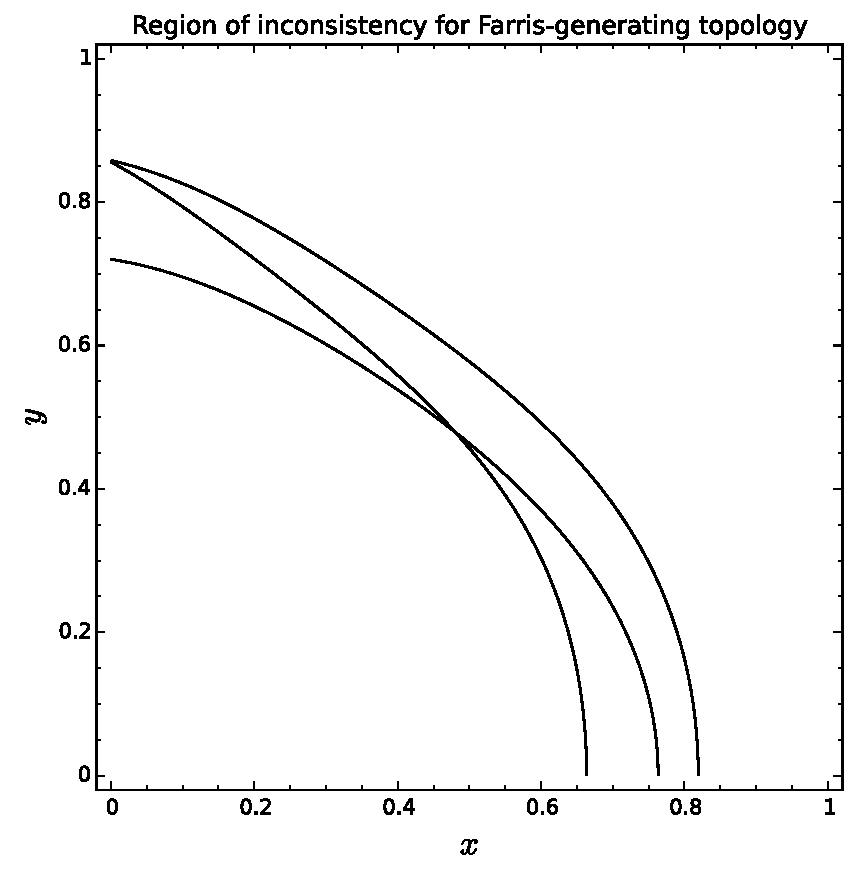
\includegraphics[width=.9\textwidth]{analytic-inconsistency}
\caption{
    Regions of inconsistency.
    Due to the looseness of the upper and lower bounds, the parameters in the top right do not necessarily indicate consistency, though all parameters in the labeled region result in an inconsistency.
}
\label{fig:inconsistency-farris}
\end{figure}

\section{Discussion}

Neyman-Scott paradox.

Interesting that here we are simulating on the Farris tree and end up with the Felsenstein tree.
For maximum parsimony it's the opposite \cite{Felsenstein1978-rr}.
Discussion of number of parameters of each.

However, note that \cite{Siddall1998-hq} get things going the same way, although \cite{Swofford2001-hr} show that the problem is that they didn't simulate long enough sequences.


\bibliographystyle{plain}
\bibliography{joint_inf}

\newpage

\section*{Appendix}

\subsection*{Site split formulation}
We begin by introducing ``site splits,'' which formalize the notion that a given site pattern is equally probable to its complement under the binary symmetric model.
This is a standard step in the description of the Hadamard transform (Section 8.6 of \citet{Semple2003-em}), although our approach is complicated slightly by the inclusion of ancestral states.

Since we have a finite character alphabet, for a given column $i$ there are a finite number of possible assignments of characters to tips $\alignmentColumn_i$ or internal nodes $\ancestralStateColumn_i$; this results in a simplification of likelihood calculation.
Take the tip labels of $\tau$ to be $\{1,\ldots,\nSiteRows\}$.
For likelihood calculation under the binary symmetric model, we describe a given $\alignmentColumn_i$ as a subset of indices $\siteSplit\subseteq\siteSplitSet:=\{1,\ldots,\nSiteRows-1\}$ with equivalent characters, commonly called a ``site split.''
We define the site split $\siteSplit$ for a $\alignmentColumn_i$ as simply $\alignmentColumn_i$ if the label $\nSiteRows$ is not in $\alignmentColumn_i$, and as its complement otherwise.
Taking such a complement simplifies but does not change the result of likelihood computation because the probability of observing a particular collection of binary characters is equivalent to the probability of its complement under the binary symmetric model.

For topology $\tau$, we define an ordered set of internal node labels $\{1,\ldots,\nAncestralStateRows\}$ for $\ancestralStateColumn_i$ and similarly use a subset of characters $\ancestralSplit\subseteq\ancestralSplitSet:=\{1,\ldots,\nAncestralStateRows\}$ to describe a realization $\ancestralStateColumn_i$.
In this case the entire set of internal nodes must be enumerated: the probability of observing an ancestral state split conditional on a site split is not invariant to taking its complement.

We enumerate the site splits $\siteSplit_j$ of which there are $\nSiteSplits=|\mathcal{P}(\siteSplitSet)|$ in total where $\mathcal{P}$ denotes the power set.
Similarly we enumerate ancestral splits $\ancestralSplit_k$ of which there are $\nAncestralSplits=|\mathcal{P}(\ancestralSplitSet)|$ in total.

We first fix notation.
\begin{definition}
Let the mapping from site patterns to site splits be
$$
\patternToSplit:\alphabet^\nSiteRows\rightarrow\mathcal{P}(\siteSplitSet)
$$
and the mapping from ancestral states and tip states to ancestral state splits be
$$
\ancestralToSplit:\alphabet^\nAncestralStateRows\times\alphabet^\nSiteRows\rightarrow\mathcal{P}(\ancestralSplitSet).
$$
Then, given a site pattern--valued random variable $\alignmentColumnRV$, define the random variable
$$
\siteSplitRV := \patternToSplit(\alignmentColumnRV)
$$
that takes corresponding realizations $\siteSplit_j$ for some $j$, and
$$
\ancestralSplitRV := \ancestralToSplit(\alignmentColumnRV, \ancestralStateColumnRV)
$$
for a tip state--valued random variable $\alignmentColumnRV$ and an ancestral state--valued random variable $\ancestralStateColumnRV$.
\end{definition}
The mapping $\patternToSplit$ takes the complement of site patterns to obtain a site split in $\mathcal{P}(\siteSplitSet)$.
The mapping $\ancestralToSplit$ is defined by whether the tip states have their complements taken or not: if a set of tip labels $\alignmentColumn$ is in $\siteSplitSet$, $\ancestralToSplit(\alignmentColumn, \ancestralStateColumn)$ is $\ancestralStateColumn$; otherwise, if $\alignmentColumn$ is not in $\siteSplitSet$, then the complement of $\alignmentColumn$ necessarily is in $\siteSplitSet$, and $\ancestralToSplit(\alignmentColumn, \ancestralStateColumn)$ is the complement of $\ancestralStateColumn$.

For the $i$th factor of \eqref{eq:full_likelihood},
$$
\Pr(\alignmentColumnRV=\alignmentColumn_i, \ancestralStateColumnRV=\ancestralStateColumn_i \mid \tau, t) = \Pr(\alignmentColumnRV=\alignmentColumn_i \mid \tau, t) \cdot \Pr(\ancestralStateColumnRV=\ancestralStateColumn_i \mid \alignmentColumnRV=\alignmentColumn_i, \tau, t).
$$
As a consequence of assuming a binary symmetric model, taking complements yields
\begin{align*}
    2\cdot \Pr(\alignmentColumnRV=\alignmentColumn_i \mid \tau, t) &= \Pr(\siteSplitRV=\patternToSplit(\alignmentColumn_i) \mid \tau, t) \\
                                                                 &= \Pr(\siteSplitRV=\siteSplit_j \mid \tau, t)
\end{align*}
for some $j$ and
\begin{align*}
    \Pr(\ancestralStateColumnRV=\ancestralStateColumn_i \mid \alignmentColumnRV=\alignmentColumn_i, \tau, t) &= \Pr(\ancestralSplitRV=\ancestralToSplit(\alignmentColumn_i, \ancestralStateColumn_i) \mid \siteSplitRV=\patternToSplit(\alignmentColumn_i), \tau, t).
\end{align*}
Given $(\tau, t)$, there exists an ordered list of sets $\fullAncestralSplitPartitions(\tau, t)=(\ancestralSplitPartition_1(\tau, t),\ldots,\ancestralSplitPartition_\nSiteSplits(\tau, t))$ such that any element $\xi_j$ of the $j$th component $\ancestralSplitPartition_j(\tau, t)$ satisfies
\begin{align*}
\max_{\ancestralSplit_k\in\mathcal{P}(\ancestralSplitSet)} \ \Pr(\ancestralSplitRV=\ancestralSplit_k \mid \siteSplitRV=\siteSplit_j, \tau, t) &= \Pr(\ancestralSplitRV = \xi_j \mid \siteSplitRV=\siteSplit_j, \tau, t).
\end{align*}
In other words, for the $j$th site split, $\ancestralSplitPartition_j(\tau, t)\subset\mathcal{P}(\ancestralSplitSet)$ is the set of most likely ancestral splits for that particular site split, topology and set of branch lengths, and $\xi_j$ is one of possibly many equiprobable ancestral state splits in $\ancestralSplitPartition_j(\tau, t)$.
For each $\alignmentColumn_i$, $\ancestralToSplit(\alignmentColumn_i, \cdot)$ is surjective, and from this we have
\begin{align*}
\max_{\ancestralStateColumn_i} \Pr(\ancestralSplitRV=\ancestralToSplit(\alignmentColumn_i, \ancestralStateColumn_i) \mid \siteSplitRV=\patternToSplit(\alignmentColumn_i), \tau, t) &= \Pr(\ancestralSplitRV = \xi_j \mid \siteSplitRV=\siteSplit_j, \tau, t).
\end{align*}

\subsection*{Site split likelihood}

Let $\xi_j$ be such a choice for each $1 \leq j \leq q$.
Then, the likelihood in \eqref{eq:profile_likelihood} written as a product over site patterns as opposed to sites is
\begin{align}
L_\nCols'(\tau, t; \fullAlignment) &= \max_{\fullAncestralStates} \ L_\nCols(\tau, t; \fullAlignment, \fullAncestralStates) \nonumber \\
                             &= \prod_{i=1}^{\nCols} \ \max_{\ancestralStateColumn_i} \ \Pr(\alignmentColumnRV=\alignmentColumn_i, \ancestralStateColumnRV=\ancestralStateColumn_i \mid \tau, t) \nonumber \\
                             &\propto \prod_{i=1}^{\nCols} \ \max_{\ancestralStateColumn_i} \ \Pr(\siteSplitRV=\patternToSplit(\alignmentColumn_i) \mid \tau, t) \cdot \Pr(\ancestralSplitRV=\ancestralToSplit(\alignmentColumn_i, \ancestralStateColumn_i) \mid \siteSplitRV=\patternToSplit(\alignmentColumn_i), \tau, t) \nonumber \\
                             &= \prod_{i=1}^{\nCols} \ \Pr(\siteSplitRV=\patternToSplit(\alignmentColumn_i) \mid \tau, t) \cdot \max_{\ancestralStateColumn_i} \Pr(\ancestralSplitRV=\ancestralToSplit(\alignmentColumn_i, \ancestralStateColumn_i) \mid \siteSplitRV=\patternToSplit(\alignmentColumn_i), \tau, t) \nonumber \\
                             &= \prod_{j=1}^{\nSiteSplits} \ \left[\Pr(\siteSplitRV=\siteSplit_j \mid \tau, t)\cdot \Pr(\ancestralSplitRV=\xi_j \mid \siteSplitRV=\siteSplit_j, \tau, t)\right] ^{\nCols_j(\fullAlignment)} \label{eq:site_pattern_likelihood}
\end{align}
where $\nCols_j(\fullAlignment)$ is the number of columns in $\fullAlignment$ that project to site split $\siteSplit_j$.

Let
$$
L_\nCols''(\tau, t; \fullAlignment) = \prod_{j=1}^{\nSiteSplits} \ \left[\Pr(\siteSplitRV=\siteSplit_j \mid \tau, t) \cdot \Pr(\ancestralSplitRV=\xi_j \mid \siteSplitRV=\siteSplit_j, \tau, t)\right] ^{\nCols_j(\fullAlignment)}
$$
be the final product in \eqref{eq:site_pattern_likelihood}.
Assume $\nCols$ observations are generated from a model with parameters $(\tau^*, t^*)$.
We have
\begin{equation*}
\begin{split}
&    \frac{1}{\nCols} \log L_\nCols''(\tau, t; \fullAlignment) \\
&\qquad = \sum_{j=1}^\nSiteSplits \frac{\nCols_j(\fullAlignment)}{\nCols}\cdot  \log \Pr(\siteSplitRV=\siteSplit_j, \ancestralSplitRV=\xi_j \mid \tau, t) \\
&\qquad = \sum_{j=1}^\nSiteSplits \frac{\nCols_j(\fullAlignment)}{\nCols}\cdot [\log \Pr(\siteSplitRV=\siteSplit_j \mid \tau, t) +
            \log \Pr(\ancestralSplitRV=\xi_j \mid \siteSplitRV=\siteSplit_j , \tau, t)]
\end{split}
\end{equation*}
so that, in the $\nCols\rightarrow\infty$ limit,
\begin{equation}
\begin{split}
&    \frac{1}{\nCols} \log L_\nCols''(\tau, t; \fullAlignment) \\
&\qquad \rightarrow \sum_{j=1}^\nSiteSplits \Pr(\siteSplitRV=\siteSplit_j \mid \tau^*, t^*) \cdot [\log \Pr(\siteSplitRV=\siteSplit_j \mid \tau, t) + \log \Pr(\ancestralSplitRV=\xi_j \mid \siteSplitRV=\siteSplit_j , \tau, t)]. \label{eq:site_pattern_profile_likelihood_mean}
\end{split}
\end{equation}
Define the divergence quantity
$$
\shannonDivergence_{\tau^*,t^*}(\tau,t) = \sum_{j=1}^\nSiteSplits \Pr(\siteSplitRV=\siteSplit_j \mid \tau^*, t^*)\cdot\log \Pr(\siteSplitRV=\siteSplit_j \mid \tau, t)
$$
and the partial log-likelihood
$$
\tilde{\ell}_{\tau^*,t^*}(\tau, t) = \sum_{j=1}^\nSiteSplits \Pr(\siteSplitRV=\siteSplit_j \mid \tau^*, t^*)\cdot\log \Pr(\ancestralSplitRV=\xi_j \mid \siteSplitRV = \siteSplit_j, \tau, t)
$$
so that \eqref{eq:site_pattern_profile_likelihood_mean} is
\begin{equation}
    \label{eq:log_likelihood_simplified}
    \ell_{\tau^*,t^*}(\tau, t) = \shannonDivergence_{\tau^*,t^*}(\tau,t) + \tilde{\ell}_{\tau^*,t^*}(\tau, t).
\end{equation}

\subsection*{Hadamard representation}

We state the Hadamard representation of site split generating probabilities, following Section 8.6 of \citet{Semple2003-em}.
For each edge $e$ define the edge ``fidelity'' for that edge as
$$
\theta(e) = 1-2p(e).
$$
For an even-sized subset of $Y\subseteq\mathcal{S}$, we define the path set $P(Y)$ as the set of edges in the path connecting both elements of $Y$.
For $n$ taxa, the probability of observing site split $A\in\mathcal{P}(\siteSplitSet)$ is
\begin{equation}
\label{eq:hadamard_probability}
p_A = \frac{1}{2^{n-1}} \ \sum_{Y \subseteq \mathcal{S} : |Y| \equiv 0 (\mathrm{mod} \ 2)} \ \left[(-1)^{|Y \cap A|} \ \prod_{e\in P(Y)} \ \theta(e) \right].
\end{equation}
By convention, we set $P(\emptyset)=\emptyset$ and $\prod_{e\in\emptyset} \ \theta(e) = 1$.
For notational convenience, let
$$
p_{\siteSplit_j} := \Pr(\siteSplitRV=\siteSplit_j \mid \tau_1,t),
$$
for any site split $\siteSplit_j$.
Table~\ref{tab:sitepatprob} contains calculations of site pattern probabilities for our two topologies (Fig.~\ref{fig:farris-fels-top}).

\begin{table}[ht]
\centering
\begin{tabular}{|l|l|l|l|}
    \hline
$\siteSplit_j$  & $p_{\siteSplit_j}$ &$\Pr(\siteSplitRV=\siteSplit_j \mid \tau_1,t)$&$\Pr(\siteSplitRV=\siteSplit_j \mid \tau_2,t)$\\
    \hline
    $\emptyset$ & $p_{\emptyset}$   &$1+x^2+y^2+4xyw+x^2y^2$&$1+2xy+2xyw+x^2w+y^2w+x^2y^2$\\
    $\{1\}$     & $p_{1}$   &$1-x^2+y^2-x^2y^2$&$1-x^2w+y^2w-x^2y^2$\\
    $\{2\}$     & $p_{2}$   &$1+x^2-y^2-x^2y^2$&$1+x^2w-y^2w-x^2y^2$\\
    $\{3\}$     & $p_{3}$   &$1-x^2+y^2-x^2y^2$&$1-x^2w+y^2w-x^2y^2$\\
    $\{1,2\}$   & $p_{12}$   &$1-x^2-y^2+x^2y^2$&$1+2xy-2xyw-x^2w-y^2w+x^2y^2$\\
    $\{1,3\}$   & $p_{13}$   &$1+x^2+y^2-4xyw+x^2y^2$&$1-2xy-2xyw+x^2w+y^2w+x^2y^2$\\
    $\{2,3\}$   & $p_{23}$   &$1-x^2-y^2+x^2y^2$&$1-2xy+2xyw-x^2w-y^2w+x^2y^2$\\
    $\{1,2,3\}$ & $p_{123}$   &$1+x^2-y^2-x^2y^2$&$1+x^2w-y^2w-x^2y^2$\\
    \hline
\end{tabular}
\caption{Site pattern probabilities $p_{\siteSplit_j}$ on the Farris tree $\tau_1$ and the Felsenstein tree $\tau_2$ obtained using the Hadamard transform.
All values multiplied by $1/8$.}
\label{tab:sitepatprob}
\end{table}

\subsection*{Example}
We follow with an expository example computing these probabilities and likelihoods.
Consider the fixed, binary four-taxon tree $\tau_1$ in Fig.~\ref{fig:farris-fels-top}a---this is commonly known as the ``Farris zone'' topology.
The set of all possible character assignments is
\begin{align*}
\mathcal{P}(\{1,2,3,4\}) &= \{\emptyset, \{1,2,3,4\}, \{1\}, \{2,3,4\}, \{2\}, \{1,3,4\}, \{3\}, \{1,2,4\}, \\
                         &\qquad \{1,2\}, \{3,4\}, \{1,3\}, \{2,4\}, \{2,3\}, \{1,4\}, \{1,2,3\}, \{1,4\}\}.
\end{align*}
where each set indicates the tips assigned the character $1$.
For example, $\emptyset$ is the labeling $0000$ and $\{1,3,4\}$ is the labeling $1011$.
Symmetry allows us to group adjacent pairs in $\mathcal{P}(\{1,2,3,4\})$ into equiprobable splits, letting $\siteSplitSet=\{1,2,3\}$.
The unique site splits, collapsing complements, are
\begin{align*}
    \mathcal{P}(\siteSplitSet) &= \{\emptyset, \{1\}, \{2\}, \{3\}, \{1,2\}, \{1,3\}, \{2,3\}, \{1,2,3\}\} \\
& := \{\siteSplit_1, \ldots, \siteSplit_8\}.
\end{align*}
Since we identify character complements, we do not consider the additional splits
\begin{equation*}
\begin{split}
& \mathcal{P}(\{1,2,3,4\}) \setminus \mathcal{P}(\siteSplitSet) = \\
&\qquad \{\{1,2,3,4\}, \{2,3,4\}, \{1,3,4\}, \{1,2,4\}, \{3,4\}, \{2,4\}, \{1,4\}, \{4\}\},
\end{split}
\end{equation*}
the symmetry of the binary character model allowing us to focus only on the elements of $\mathcal{P}(\siteSplitSet)$.
This tree has two internal nodes with $\ancestralSplitSet=\{1,2\}$ and unique ancestral state splits
$$
\mathcal{P}(\ancestralSplitSet) = \{\emptyset, \{1\}, \{2\}, \{1,2\}\}.
$$
Internal node $\{1\}$ is the node connected to leaves $\{1\}$ and $\{3\}$ and internal node $\{2\}$ connected to leaves $\{2\}$ and $\{4\}$.
The mapping from characters to splits in this case will depend on the characters at the tips and the ancestral states.
For example, we take both $\patternToSplit(0000)=\emptyset$ and $\patternToSplit(1111)=\emptyset$.
Similarly, we have $\ancestralToSplit(0000, 00) = \emptyset$ and $\ancestralToSplit(1111, 11)=\emptyset$, needing to take the complement of all the characters present on the tree to identify splits.
We cannot identify complements for ancestral states in the same way as tip states since, for $\siteSplit\in\mathcal{P}(\siteSplitSet)$,
$$
\Pr(\ancestralSplitRV=\emptyset \mid \siteSplitRV=\siteSplit, \tau, t)\neq \Pr(\ancestralSplitRV=\{1,2\} \mid \siteSplitRV=\siteSplit, \tau, t)
$$
in general.

For each site split $\siteSplit\in\mathcal{P}(\siteSplitSet)$, we maximize the likelihood over all $\ancestralSplit\in\mathcal{P}(\ancestralSplitSet)$.
A maximum occurs at one of possibly several ancestral splits in $\mathcal{P}(\ancestralSplitSet)$, defined via $\ancestralSplitPartition_j(\tau, t)$ for the $j$th site split.
As a simple example, say all branch lengths correspond to a probability $p$ ($< 1/2$) of changing character along that branch, with $t=\{p,p,p,p,p\}$.
The probabilities of observing ancestral splits for $\siteSplit_1=\emptyset$ are
$$
\Pr(\ancestralSplitRV=\emptyset \mid \siteSplitRV=\emptyset, \tau, t) =
(1-p)^5,
$$
$$
\Pr(\ancestralSplitRV=\{1\} \mid \siteSplitRV=\emptyset, \tau, t) =
\Pr(\ancestralSplitRV=\{2\} \mid \siteSplitRV=\emptyset, \tau, t) =
p^3(1-p)^2,
$$
$$
\Pr(\ancestralSplitRV=\{1,2\} \mid \siteSplitRV=\emptyset, \tau, t) =
p^4(1-p).
$$
The set of most likely ancestral states contains a single element, here $\ancestralSplitPartition_1(\tau, t)=\{\emptyset\}$.
Then, taking $\xi_1\in\ancestralSplitPartition_1(\tau, t)$ we have
$$
\Pr(\ancestralSplitRV=\xi_1 \mid \siteSplitRV=\emptyset, \tau, t) =
\Pr(\ancestralSplitRV=\emptyset \mid \siteSplitRV=\emptyset, \tau, t) =
(1-p)^5.
$$
For $\siteSplit_5=\{1,2\}$ we have
$$
\Pr(\ancestralSplitRV=\emptyset \mid \siteSplitRV=\{1,2\}, \tau, t) =
\Pr(\ancestralSplitRV=\{1,2\} \mid \siteSplitRV=\{1,2\}, \tau, t) =
p^2(1-p)^3,
$$
$$
\Pr(\ancestralSplitRV=\{1\} \mid \siteSplitRV=\{1,2\}, \tau, t) =
\Pr(\ancestralSplitRV=\{2\} \mid \siteSplitRV=\{1,2\}, \tau, t) =
p^3(1-p)^2.
$$
Here, the set of most likely ancestral states is $\ancestralSplitPartition_5(\tau, t)=\{\emptyset,\{1,2\}\}$, and, for $\xi_5\in\ancestralSplitPartition_5(\tau, t)$,
$$
\Pr(\ancestralSplitRV=\xi_5 \mid \siteSplitRV=\{1,2\}, \tau, t) =
p^2(1-p)^3.
$$

\subsection*{Likelihood computations}

To compute the likelihood of observing a set of data, we need $\Pr(\ancestralStateColumn=\ancestralSplit_k\mid \alignmentColumn=\siteSplit_j,\tau,t)$ for each $\ancestralSplit_k$ and $\siteSplit_j$.
Using branch fidelities, the probability of a character change along a branch with fidelity parameter $\theta$ is $(1-\theta)/2$, while the probability of a character remaining the same is $(1+\theta)/2$.
See Fig.~\ref{fig:example_likelihoods} for the parameters on an example site pattern on the Farris tree.
Likelihood computations for all site patterns and ancestral states are in Tables~\ref{tab:farris_likelihoods} and~\ref{tab:fels_likelihoods}.
Taking maxima row-wise of each table results in Table~\ref{tab:likelihoods}.

\begin{figure}
\centering
\begin{subfigure}{.45\linewidth}
\centering
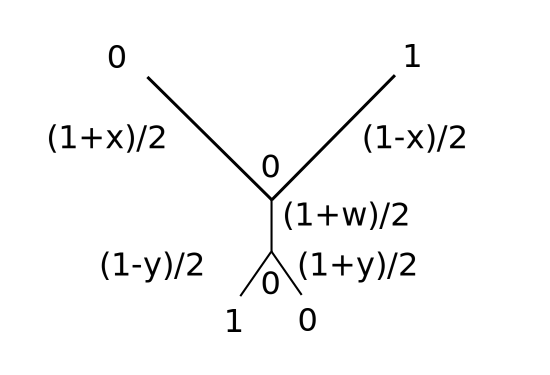
\includegraphics[width=.95\textwidth]{farris_like00}
\caption[short]{}
\end{subfigure}
\begin{subfigure}{.45\linewidth}
\centering
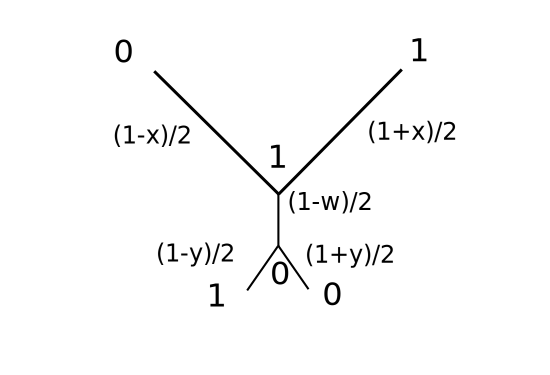
\includegraphics[width=.95\textwidth]{farris_like10}
\caption[short]{}
\end{subfigure}
\caption{
    Example likelihood computations on the Farris tree $\tau_1$ for fidelities $x$, $y$, and $w$.
    Edges labeled by the probability of substitution along that edge.
    In (a), we compute the product to obtain $\Pr(\ancestralStateColumn=\emptyset\mid \alignmentColumn=\{2,3\},\tau_1,t) = (1+x)(1-x)(1+y)(1-y)(1+w)/32$.
    In (b), the same process yields $\Pr(\ancestralStateColumn=\{1\}\mid \alignmentColumn=\{2,3\},\tau_1,t) = (1+x)(1-x)(1+y)(1-y)(1-w)/32$.
}
\label{fig:example_likelihoods}
\end{figure}

\begin{table}
\centering
\begin{tabular}{|l|ll|}
\multicolumn{3}{c}{$\Pr(\ancestralStateColumn=\ancestralSplit_k\mid \alignmentColumn=\siteSplit_j,\tau_1,t)$}\\
\hline
& \multicolumn{2}{|c|}{$\ancestralSplit_k$}\\
    \hline
    $\siteSplit_j$    &$\emptyset$                                &$\{2\}$  \\
    \hline
     $\emptyset$   &$(1+x)^2   (1+w)(1+y)^2$          &$(1+x)^2   (1-w)(1-y)^2$\\
     $\{1\}$       &$(1+x)(1-x)(1+w)(1+y)^2$          &$(1+x)(1-x)(1-w)(1-y)^2$\\
     $\{2\}$       &$(1+x)^2   (1+w)(1+y)(1-y)$       &$(1+x)^2   (1-w)(1+y)(1-y)$\\
     $\{3\}$       &$(1+x)(1-x)(1+w)(1+y)^2$          &$(1+x)(1-x)(1-w)(1-y)^2$\\
     $\{1,2\}$     &$(1+x)(1-x)(1+w)(1+y)(1-y)$       &$(1+x)(1-x)(1-w)(1+y)(1-y)$\\
     $\{1,3\}$     &$(1-x)^2   (1+w)(1+y)^2$          &$(1-x)^2   (1-w)(1-y)^2$\\
     $\{2,3\}$     &$(1+x)(1-x)(1+w)(1+y)(1-y)$       &$(1+x)(1-x)(1-w)(1+y)(1-y)$\\
     $\{1,2,3\}$   &$(1-x)^2   (1+w)(1+y)(1-y)$       &$(1-x)^2   (1-w)(1+y)(1-y)$\\
    \hline
    \hline
    &$\{1\}$                             &$\{1,2\}$  \\
    \hline
     $\emptyset$   &$(1-x)^2   (1-w)(1+y)^2$     &$(1-x)^2   (1+w)(1-y)^2$\\
     $\{1\}$       &$(1+x)(1-x)(1-w)(1+y)^2$     &$(1+x)(1-x)(1+w)(1-y)^2$\\
     $\{2\}$       &$(1-x)^2   (1-w)(1+y)(1-y)$  &$(1-x)^2   (1+w)(1+y)(1-y)$\\
     $\{3\}$       &$(1+x)(1-x)(1-w)(1+y)^2$     &$(1+x)(1-x)(1+w)(1-y)^2$\\
     $\{1,2\}$     &$(1+x)(1-x)(1-w)(1+y)(1-y)$  &$(1+x)(1-x)(1+w)(1+y)(1-y)$\\
     $\{1,3\}$     &$(1+x)^2   (1-w)(1+y)^2$     &$(1+x)^2   (1+w)(1-y)^2$\\
     $\{2,3\}$     &$(1+x)(1-x)(1-w)(1+y)(1-y)$  &$(1+x)(1-x)(1+w)(1+y)(1-y)$\\
     $\{1,2,3\}$   &$(1+x)^2   (1-w)(1+y)(1-y)$  &$(1+x)^2   (1+w)(1+y)(1-y)$\\
    \hline
\end{tabular}
\caption{Likelihood calculations for all site patterns $\siteSplit_j$ and internal states $\ancestralSplit_k$ of the Farris tree $\tau_1$.
All values multiplied by $1/32$.}
\label{tab:farris_likelihoods}
\end{table}

\begin{table}
\centering
\begin{tabular}{|l|ll|}
\multicolumn{3}{c}{$\Pr(\ancestralStateColumn=\ancestralSplit_k\mid \alignmentColumn=\siteSplit_j,\tau_2,t)$}\\
\hline
& \multicolumn{2}{|c|}{$\ancestralSplit_k$}\\
    \hline
    $\siteSplit_j$    &$\emptyset$                                &$\{2\}$  \\
    \hline
     $\emptyset$   &$(1+x)^2   (1+w)(1+y)^2$           &$(1+x)(1-x)(1-w)(1+y)(1-y)$\\
     $\{1\}$       &$(1+x)(1-x)(1+w)(1+y)^2$           &$(1-x)^2   (1-w)(1+y)(1-y)$\\
     $\{2\}$       &$(1+x)^2   (1+w)(1+y)(1-y)$        &$(1+x)(1-x)(1-w)(1-y)^2$\\
     $\{3\}$       &$(1+x)(1-x)(1+w)(1+y)^2$           &$(1+x)^2   (1-w)(1+y)(1-y)$\\
     $\{1,2\}$     &$(1+x)(1-x)(1+w)(1+y)(1-y)$        &$(1-x)^2   (1-w)(1-y)^2$\\
     $\{1,3\}$     &$(1-x)^2   (1+w)(1+y)^2$           &$(1+x)(1-x)(1-w)(1+y)(1-y)$\\
     $\{2,3\}$     &$(1+x)(1-x)(1+w)(1+y)(1-y)$        &$(1+x)^2   (1-w)(1-y)^2$\\
     $\{1,2,3\}$   &$(1-x)^2   (1+w)(1+y)(1-y)$        &$(1+x)(1-x)(1-w)(1-y)^2$\\
    \hline
    \hline
    &$\{1\}$                             &$\{1,2\}$  \\
    \hline
     $\emptyset$   &$(1+x)(1-x)(1-w)(1+y)(1-y)$        &$(1-x)^2   (1+w)(1-y)^2$\\
     $\{1\}$       &$(1+x)^2   (1-w)(1+y)(1-y)$        &$(1+x)(1-x)(1+w)(1-y)^2$\\
     $\{2\}$       &$(1+x)(1-x)(1-w)(1+y)^2$           &$(1-x)^2   (1+w)(1+y)(1-y)$\\
     $\{3\}$       &$(1-x)^2   (1-w)(1+y)(1-y)$        &$(1+x)(1-x)(1+w)(1-y)^2$\\
     $\{1,2\}$     &$(1+x)^2   (1-w)(1+y)^2$           &$(1+x)(1-x)(1+w)(1+y)(1-y)$\\
     $\{1,3\}$     &$(1+x)(1-x)(1-w)(1+y)(1-y)$        &$(1+x)^2   (1+w)(1-y)^2$\\
     $\{2,3\}$     &$(1-x)^2   (1-w)(1+y)^2$           &$(1+x)(1-x)(1+w)(1+y)(1-y)$\\
     $\{1,2,3\}$   &$(1+x)(1-x)(1-w)(1+y)^2$           &$(1+x)^2   (1+w)(1+y)(1-y)$\\
\hline
\end{tabular}
\caption{Likelihood calculations for all site patterns $\siteSplit_j$ and internal states $\ancestralSplit_k$ of the Felsenstein tree $\tau_2$.
All values multiplied by $1/32$.}
\label{tab:fels_likelihoods}
\end{table}

\begin{table}
\centering
\begin{tabular}{|l|ll|}
    \multicolumn{3}{c}{Farris tree ($\tau=\tau_1$)}\\
    \hline
    $\siteSplit_j$    & $\ancestralSplitPartition_j(\tau, t)$ & $\Pr(\ancestralSplitRV=\xi_j \mid \siteSplitRV=\siteSplit_j,\tau,t)$\\
    \hline
    $\emptyset$&
    $\emptyset$&
    $(1+x)^2   (1+w)(1+y)^2$\\
     $\{1\}$    &
    $\emptyset$&
    $(1+x)(1-x)(1+w)(1+y)^2$\\
     $\{2\}$    &
    $\emptyset$&
    $(1+x)^2   (1+w)(1+y)(1-y)$\\
     $\{3\}$    &
    $\emptyset$&
    $(1+x)(1-x)(1+w)(1+y)^2$\\
    $\{1,2\}$  &
    $\{\emptyset,\{1,2\}\}$&
    $(1+x)(1-x)(1+w)(1+y)(1-y)$\\
    $\{1,3\}$  &
    $\left\{\begin{array}{l}
                    \emptyset\\
                    \{1\}\\
                    \{1,2\}
                \end{array}\right.$&
    $\begin{array}{l}
                    (1-x)^2   (1+w)(1+y)^2\\
                    (1+x)^2   (1-w)(1+y)^2\\
                    (1+x)^2   (1+w)(1-y)^2
                \end{array}$\\
    $\{2,3\}$  &
                $\{\emptyset,\{1,2\}\}$&
                $(1+x)(1-x)(1+w)(1+y)(1-y)$\\
    $\{1,2,3\}$&
                $\{1,2\}$&
                $(1+x)^2   (1+w)(1+y)(1-y)$\\
    \hline
    \multicolumn{3}{c}{Felsenstein tree ($\tau=\tau_2$)}\\
    \hline
    $\siteSplit_j$    & $\ancestralSplitPartition_j(\tau, t)$ & $\Pr(\ancestralSplitRV=\xi_j \mid \siteSplitRV=\siteSplit_j,\tau,t)$\\
    \hline
    $\emptyset$       &$\emptyset$&$(1+x)^2   (1+w)(1+y)^2$\\
    $\{1\}$          &
    $\left\{\begin{array}{l}
                    \emptyset\\
                    \{1\}
                \end{array}\right.$&
    $\begin{array}{l}
                        (1+x)(1-x)(1+w)(1+y)^2\\
                        (1+x)^2   (1-w)(1+y)(1-y)
                    \end{array}$\\
      $\{2\}$          &
    $\left\{\begin{array}{l}
                    \emptyset\\
                    \{1\}
                \end{array}\right.$&
    $\begin{array}{l}
                    (1+x)^2   (1+w)(1+y)(1-y)\\
                    (1+x)(1-x)(1-w)(1+y)^2
                    \end{array}$\\
      $\{3\}$          &
    $\left\{\begin{array}{l}
                    \emptyset\\
                    \{2\}
                \end{array}\right.$&
    $\begin{array}{l}
                    (1+x)(1-x)(1+w)(1+y)^2\\
                    (1+x)^2   (1-w)(1+y)(1-y)
                    \end{array}$\\
     $\{1,2\}$         &
    $\left\{\begin{array}{l}
                    \{\emptyset,\{1,2\}\}\\
                    \{1\}
                \end{array}\right.$&
    $\begin{array}{l}
                    (1+x)(1-x)(1+w)(1+y)(1-y)\\
                    (1+x)^2   (1-w)(1+y)^2
                    \end{array}$\\
     $\{1,3\}$         &
    $\left\{\begin{array}{l}
                    \emptyset\\
                    \{\{1\},\{2\}\}\\
                    \{1,2\}
                \end{array}\right.$&
    $\begin{array}{l}
                    (1-x)^2   (1+w)(1+y)^2\\
                    (1+x)(1-x)(1-w)(1+y)(1-y)\\
                    (1+x)^2   (1+w)(1-y)^2
                    \end{array}$\\
      $\{2,3\}$        &
    $\left\{\begin{array}{l}
                    \{\emptyset,\{1,2\}\}\\
                    \{1\}\\
                    \{2\}
                \end{array}\right.$&
    $\begin{array}{l}
                    (1+x)(1-x)(1+w)(1+y)(1-y)\\
                    (1-x)^2   (1-w)(1+y)^2\\
                    (1+x)^2   (1-w)(1-y)^2
                    \end{array}$\\
     $\{1,2,3\}$       &
    $\left\{\begin{array}{l}
                    \{2\} \\
                    \{1,2\}
                \end{array}\right.$&
    $\begin{array}{l}
                    (1+x)(1-x)(1-w)(1+y)^2 \\
                    (1+x)^2   (1+w)(1+y)(1-y)
                    \end{array}$\\
    \hline
\end{tabular}
\caption{Likelihood calculations for all site patterns $\siteSplit_j$ and ancestral state partitions $\ancestralSplitPartition_j$ after maximizing over ancestral states on the Farris tree $\tau_1$ and the Felsenstein tree $\tau_2$.
All values multiplied by $1/32$.
Likelihoods with multiple entries have maxima determined by unknown branch length parameters.
See Tables~\ref{tab:farris_likelihoods} and~\ref{tab:fels_likelihoods} for full calculations.}
\label{tab:likelihoods}
\end{table}

\subsection*{Form of the likelihood}

Consider the Farris tree with arbitrary fidelities, i.e., $\tilde{t}=\{x_1,y_1,x_2,y_2,w\}$.
We now show that, in the case of the Farris tree, exchanging $x_1$ with $x_2$ and $y_1$ with $y_2$ does not change the value of the likelihood, and that constraining both the top two branch parameters to be equal and the bottom two branch parameters to be equal during inference obtains the same maximum likelihood estimate as in the case of arbitrary branch parameters.
Using the Hadamard transform, we calculate the generating probabilities on the Farris tree.
For site split $\emptyset$,
\begin{align*}
    \Pr(\siteSplitRV=\emptyset\mid \tau_1, \tilde{t}) & = \frac{1}{8} (1 + x_1x_2 +  y_1y_2 +  x_1y_1w + x_1y_2w + y_1x_2w + x_2y_2w + x_1y_1x_2y_2) \\
                                              & = \frac{1}{8} (1 + x_1x_2 +  y_1y_2 +  w[x_1y_1 + x_1y_2 + y_1x_2 + x_2y_2] + x_1y_1x_2y_2) \\
                                              & = \frac{1}{8} (1 + x_1x_2 +  y_1y_2 +  w[x_1 + x_2][y_1 + y_2] + x_1y_1x_2y_2).
\end{align*}
and this probability is unchanged when $x_1$ is exchanged with $x_2$ and $y_1$ is exchanged with $y_2$.
All other generating probabilities will differ only in the signs of each term.
For example, for site split $\{1\}$ we have
\begin{align*}
    \Pr(\siteSplitRV=\{1\}\mid \tau_1, \tilde{t}) & = \frac{1}{8} (1 - x_1x_2 +  y_1y_2 +  w[-x_1 + x_2][y_1 + y_2] - x_1y_1x_2y_2)
\end{align*}
and for site split $\{3\}$ we have
\begin{align*}
    \Pr(\siteSplitRV=\{3\}\mid \tau_1, \tilde{t}) & = \frac{1}{8} (1 - x_1x_2 +  y_1y_2 +  w[x_1 - x_2][y_1 + y_2] - x_1y_1x_2y_2)
\end{align*}
meaning if we exchange the values of $x_1$ and $x_2$ then these probabilities swap values.
The corresponding possibilities for the likelihood values are
\begin{align*}
    \Pr(\ancestralSplitRV=\emptyset \mid \siteSplitRV=\{1\}, \tau_1, \tilde{t}) &= \frac{1}{32}(1-x_1)(1+x_2)(1+w)(1+y_1)(1+y_2); \\
    \Pr(\ancestralSplitRV=\{1\} \mid \siteSplitRV=\{1\}, \tau_1, \tilde{t}) &= \frac{1}{32}(1+x_1)(1-x_2)(1-w)(1+y_1)(1+y_2); \\
    \Pr(\ancestralSplitRV=\{2\} \mid \siteSplitRV=\{1\}, \tau_1, \tilde{t}) &= \frac{1}{32}(1-x_1)(1+x_2)(1-w)(1-y_1)(1-y_2); \\
    \Pr(\ancestralSplitRV=\{1,2\} \mid \siteSplitRV=\{1\}, \tau_1, \tilde{t}) &= \frac{1}{32}(1+x_1)(1-x_2)(1+w)(1-y_1)(1-y_2);
\end{align*}
for site split $\{1\}$ and
\begin{align*}
        \Pr(\ancestralSplitRV=\emptyset \mid \siteSplitRV=\{3\}, \tau_1, \tilde{t}) &= \frac{1}{32}(1+x_1)(1-x_2)(1+w)(1+y_1)(1+y_2); \\
    \Pr(\ancestralSplitRV=\{1\} \mid \siteSplitRV=\{3\}, \tau_1, \tilde{t}) &= \frac{1}{32}(1-x_1)(1+x_2)(1-w)(1+y_1)(1+y_2); \\
    \Pr(\ancestralSplitRV=\{2\} \mid \siteSplitRV=\{3\}, \tau_1, \tilde{t}) &= \frac{1}{32}(1+x_1)(1-x_2)(1-w)(1-y_1)(1-y_2); \\
    \Pr(\ancestralSplitRV=\{1,2\} \mid \siteSplitRV=\{3\}, \tau_1, \tilde{t}) &= \frac{1}{32}(1-x_1)(1+x_2)(1+w)(1-y_1)(1-y_2);
\end{align*}
for site split $\{3\}$, which also both swap values when $x_1$ and $x_2$ are exchanged.

The same can be done for the splits $\{2\}$ and $\{1,2,3\}$ by exchanging $y_1$ and $y_2$ as well as $\{1,2\}$ and $\{1,3\}$ by exchanging both $x_1$ with $x_2$ and $y_1$ with $y_2$.
The split $\{1,3\}$ is unchanged by exchanging $x_1$ with $x_2$ and $y_1$ with $y_2$.

Since exchanging $x_1$ and $x_2$ does not change the value of the log-likelihood $\ell_{\tau_1,t^*}(\tau_1, \tilde{t})$, if there is a unique maximum of the log-likelihood we will have $x_1=x_2$ at the maximum.
An analogous statement holds for $y_1$ and $y_2$.
It remains to show that the joint inference procedure maximizing \eqref{eq:profile_likelihood} results in a unique estimate of $t$.
Without loss of generality, we focus on the single parameter $x_1$ and show we obtain a unique maximum when performing joint inference; similar arguments hold for the remaining parameters.
We decompose the likelihood into the entropy and partial likelihood terms as in \eqref{eq:log_likelihood_simplified}.
By Gibbs's inequality, the entropy term $\shannonDivergence_{\tau^*,t^*}(\tau^*,t)$ has a unique maximum over $t$---namely $t^*$.
For the general case of $\tilde{t}=\{x_1, y_2, x_1, y_2, w\}$, we can compute the partial likelihood $\tilde{\ell}_{\tau^*,t^*}(\tau^*, t)$ as in Table~\ref{tab:farris_likelihoods}.
Clearly this partial likelihood will be of the form $g(x_1) = p\log(1+x_1) + (1-p)\log(1-x_1)$ with $0 \le p \le 1$, which, by the second derivative test, is concave for $x_1\in[0,1]$ and thus has a unique maximum.
Since both summands of the likelihood are concave on $x_1\in[0,1]$, the likelihood is as well, and there exists a single $x_1\in[0,1]$ maximizing the likelihood.
Given this and the symmetry of the likelihood, we let $x_1=x_2=x$ and $y_1=y_2=y$.
The Felsenstein tree does not admit this property, but, since we are interested in a lower bound for this tree, we simplify the objective function by constraining $x_1=x_2$ and $y_1=y_2$ similarly.

\subsection*{Theorems and proofs}

\topoInconsist*

\begin{proof}
In general,
$$
\max_{t} \ \ell_{\tau^*,t^*}(\tau, t) \le
    \shannonDivergence_{\tau^*,t^*}(\tau^*,t^*)
    + \tilde{\ell}_{\tau^*,t^*}(\tau, \hat{t})
$$
is an upper bound for the joint maximum of \eqref{eq:log_likelihood_simplified} using Gibbs's inequality
$$
\shannonDivergence_{\tau^*,t^*}(\tau,t) \le \shannonDivergence_{\tau^*,t^*}(\tau^*,t^*)
$$
and
$$
\hat{t} = \argmax_{t} \ \tilde{\ell}_{\tau^*,t^*}(\tau, t).
$$
Similarly,
$$
\max_{t} \ \ell_{\tau^*,t^*}(\tau, t) \ge
    \shannonDivergence_{\tau^*,t^*}(\tau,\hat{t})
    + \tilde{\ell}_{\tau^*,t^*}(\tau, \hat{t})
$$
is a lower bound.

Assume $\tau^*=\tau_1$.
The Farris tree log-likelihood takes one of three values depending on branch lengths, which is due to site split $\{1,3\}$ (see the upper table of Table~\ref{tab:likelihoods}).

We write out the case for the ancestral state split $\{1\}$, and show the other two cases follow a similar argument.
Directly substituting calculations from Table~\ref{tab:sitepatprob} and Table~\ref{tab:likelihoods} where $\tau = \tau_1$ in \eqref{eq:site_pattern_profile_likelihood_mean}, the log-likelihood is, suppressing normalizing constants $-\log 8$ (from the first additive term of \eqref{eq:site_pattern_profile_likelihood_mean}) and $-\log 32$ (from the second),
\begin{align}
    \label{eq:farris_likelihood}
    \ell_{\tau_1,t^*}(\tau_1, t)
    &=        p_{\emptyset}  \cdot\log(1+x^2+y^2+4xyw+x^2y^2) \nonumber \\
    &\qquad + p_{1}          \cdot\log(1-x^2+y^2-x^2y^2) \nonumber \\
    &\qquad + p_{2}          \cdot\log(1+x^2-y^2-x^2y^2) \nonumber \\
    &\qquad + p_{3}          \cdot\log(1-x^2+y^2-x^2y^2) \nonumber \\
    &\qquad + p_{12}         \cdot\log(1-x^2-y^2+x^2y^2) \nonumber \\
    &\qquad + p_{13}         \cdot\log(1+x^2+y^2-4xyw+x^2y^2) \nonumber \\
    &\qquad + p_{23}         \cdot\log(1-x^2-y^2+x^2y^2) \nonumber \\
    &\qquad + p_{123}        \cdot\log(1+x^2-y^2-x^2y^2) \nonumber \\
    &\qquad + p_{\emptyset}  \cdot\log((1+x)^2   (1+w)(1+y)^2) \nonumber \\
    &\qquad + p_{1}          \cdot\log((1+x)(1-x)(1+w)(1+y)^2) \nonumber \\
    &\qquad + p_{2}          \cdot\log((1+x)^2   (1+w)(1+y)(1-y)) \nonumber \\
    &\qquad + p_{3}          \cdot\log((1+x)(1-x)(1+w)(1+y)^2) \nonumber \\
    &\qquad + p_{12}         \cdot\log((1+x)(1-x)(1+w)(1+y)(1-y)) \nonumber \\
    &\qquad + p_{13}         \cdot\log((1+x)^2   (1-w)(1+y)^2) \nonumber \\
    &\qquad + p_{23}         \cdot\log((1+x)(1-x)(1+w)(1+y)(1-y)) \nonumber \\
    &\qquad + p_{123}        \cdot\log((1+x)^2   (1+w)(1+y)(1-y)).
\end{align}
Our plan is to simplify the likelihood to remove log-of-quadratic terms of $x,y,$ and $w$, obtaining a likelihood that has a closed-form maximum in each variable.
To bound the generating probabilities, we use the facts that, for $x,y\in[0,1]$,
\begin{align*}
p_{12} = p_{23} = 1-x^2-y^2+x^2y^2 & = (1+x)(1-x)(1+y)(1-y) \\
p_{1} = p_{3} = 1-x^2+y^2-x^2y^2 & = (1+x)(1-x)(1+y^2) \le (1+x)(1-x)(1+y) \\
p_{2} = p_{123} = 1+x^2-y^2-x^2y^2 & = (1+x^2)(1+y)(1-y) \le (1+x)(1+y)(1-y).
\end{align*}
To bound the remaining $p_{\emptyset}$ and $p_{13}$, we use
\begin{align*}
1+x^2+y^2+x^2y^2 & = (1+x^2)(1+y^2) \le (1+x)(1+y) \\
4xy & = 2x \cdot 2y \le (1+x^2)(1+y^2) \le (1+x)(1+y)
\end{align*}
so that the $p_{\emptyset}$ term is bounded as
\begin{align*}
    p_{\emptyset} & = \log(1+x^2+y^2+4xyw+x^2y^2) \\
                  & \le \log(1+x^2+y^2+4xy+x^2y^2) \\
                  & \le \log(2(1+x)(1+y))
\end{align*}
and $p_{13}$ is bounded as
\begin{align*}
    p_{13} & = \log(1+x^2+y^2-4xyw+x^2y^2) \\
                  & \le \log(1+x^2+y^2+x^2y^2) \\
                  & \le \log((1+x)(1+y)).
\end{align*}
Factoring and making these substitutions (again, under the assumption that the ancestral state split is $\{1\}$) results in
\begin{align*}
&    \ell_{\tau_1,t^*}(\tau_1, t) \\
&\qquad \le      p_{\emptyset}  \cdot\log(2(1+x)(1+y))
+ p_{1}          \cdot\log((1+x)(1-x)(1+y)) \\
    &\qquad\qquad + p_{2}          \cdot\log((1+x)(1+y)(1-y))
+ p_{3}          \cdot\log((1+x)(1-x)(1+y)) \\
    &\qquad\qquad + p_{12}         \cdot\log((1+x)(1-x)(1+y)(1-y))
+ p_{13}         \cdot\log((1+x)(1+y)) \\
    &\qquad\qquad + p_{23}         \cdot\log((1+x)(1-x)(1+y)(1-y))
+ p_{123}        \cdot\log((1+x)(1+y)(1-y)) \\
    &\qquad\qquad + p_{\emptyset}  \cdot\log((1+x)^2   (1+w)(1+y)^2)
+ p_{1}          \cdot\log((1+x)(1-x)(1+w)(1+y)^2) \\
    &\qquad\qquad + p_{2}          \cdot\log((1+x)^2   (1+w)(1+y)(1-y))
+ p_{3}          \cdot\log((1+x)(1-x)(1+w)(1+y)^2) \\
    &\qquad\qquad + p_{12}         \cdot\log((1+x)(1-x)(1+w)(1+y)(1-y))
+ p_{13}         \cdot\log((1+x)^2   (1-w)(1+y)^2) \\
    &\qquad\qquad + p_{23}         \cdot\log((1+x)(1-x)(1+w)(1+y)(1-y))
+ p_{123}        \cdot\log((1+x)^2   (1+w)(1+y)(1-y)) \\
&\qquad =      p_{\emptyset}  \cdot\log(2)
+ \log(1+x)
+ (p_{1}+p_{3}+p_{12}+p_{23})\cdot\log(1-x) \\
&\qquad\qquad + \log(1+y)
+ (p_{2}+p_{12}+p_{23}+p_{123})\cdot\log(1-y) \\
&\qquad\qquad + (2-p_{1}-p_{3}-p_{12}-p_{23})\cdot\log(1+x)
+ (p_{1}+p_{3}+p_{12}+p_{23})\cdot\log(1-x) \\
&\qquad\qquad + (2-p_{2}-p_{12}-p_{23}-p_{123})\cdot\log(1+y)
+ (p_{2}+p_{12}+p_{23}+p_{123})\cdot\log(1-y) \\
&\qquad\qquad + (1-p_{13})\cdot\log(1+w)
+ p_{13}\cdot\log(1-w) \\
&\qquad =      p_{\emptyset}  \cdot\log(2)
+ (3-p_{1}-p_{3}-p_{12}-p_{23})\cdot\log(1+x)
+ 2(p_{1}+p_{3}+p_{12}+p_{23})\cdot\log(1-x) \\
&\qquad\qquad + (3-p_{2}-p_{12}-p_{23}-p_{123})\cdot\log(1+y)
+ 2(p_{2}+p_{12}+p_{23}+p_{123})\cdot\log(1-y) \\
&\qquad\qquad + (1-p_{13})\cdot\log(1+w)
+ p_{13}\cdot\log(1-w).
\end{align*}
To simplify, let
\begin{equation}
    \begin{aligned}
        a_{1} &= 3-p_{1}-p_{3}-p_{12}-p_{23}, \\
        a_{2} &= 2(p_{1}+p_{3}+p_{12}+p_{23}), \\
        a_{3} &= 3-p_{2}-p_{12}-p_{23}-p_{123}, \\
        a_{4} &= 2(p_{2}+p_{12}+p_{23}+p_{123}), \\
    \end{aligned}
    \label{eq:a_const}
\end{equation}
so that
\begin{equation*}
\begin{split}
&    \ell_{\tau_1,t^*}(\tau_1, t) \\
&\qquad \le      p_{\emptyset}  \cdot\log(2)
+ a_{1}\cdot\log(1+x)
+ a_{2}\cdot\log(1-x)
+ a_{3}\cdot\log(1+y) \\
&\qquad\qquad + a_{4}\cdot\log(1-y)
+ (1-p_{13})\cdot\log(1+w)
+ p_{13}\cdot\log(1-w).
\end{split}
\end{equation*}
Maximizing over the unknown terms yields
$$
\hat{x} = \frac{a_{1}-a_{2}}{a_{1}+a_{2}}, \ \hat{y} = \frac{a_{3}-a_{4}}{a_{3}+a_{4}}, \ \hat{w} = 1-2p_{13}.
$$
Trivially $0 \le \hat{w} \le 1$ and $\hat{x}, \hat{y} \le 1$.
We check that $\hat{x}, \hat{y} \ge 0$ to ensure these maxima are valid.
For $\hat{x} \ge 0$ we need $a_1 \ge a_2$; letting
$$
\tilde{p} = p_{1}+p_{3}+p_{12}+p_{23}
$$
we have from \eqref{eq:a_const} that $a_1 \ge a_2$ only if $3 \ge 3\tilde{p}$.
Since $\tilde{p} = 1/8\cdot(4-4(x^*)^2)$, we have $0 \le \tilde{p} \le 1/2$ implying $\hat{x} \ge 0$.
The same approach works for $\hat{y}$.
The upper bound for the likelihood is then maximized at
\begin{align}
\begin{split}
&    \ell_{\tau_1,t^*}(\tau_1, t) \\
&\qquad\le      p_{\emptyset}  \cdot\log(2)
+ a_{1}\cdot\log\frac{2a_{1}}{a_{1}+a_{2}}
+ a_{2}\cdot\log\frac{2a_{2}}{a_{1}+a_{2}}
+ a_{3}\cdot\log\frac{2a_{3}}{a_{3}+a_{4}} \\
&\qquad\qquad + a_{4}\cdot\log\frac{2a_{4}}{a_{3}+a_{4}}
+ (1-p_{13})\cdot\log(2(1-p_{13}))
+ p_{13}\cdot\log(2p_{13}) \\
&\qquad := C^{1}_{\tau_1,\tau_1}(x^*, y^*).
\end{split}
\label{eq:farris-upper-bound}
\end{align}

The other two possible ancestral state splits for the likelihood of the site split $\{1,3\}$ admit similar simplifications.
The upper bound in \eqref{eq:farris-upper-bound} is for the ancestral state split $\{1\}$.
For the ancestral state split $\emptyset$ we see the upper bound will be the same except we lose a $(1+x)^2$ term, gain a $(1-x)^2$ term, lose a $(1-w)$ term, and gain a $(1+w)$ term.
In this case, all terms involving $w$ simplify to $\log(1+w)$, maximized at $\hat{w}=1$.
For the constants above, $a_{1}$ is the multiplier for the $\log(1+x)$ term and $a_{2}$ for the $\log(1-x)$ term meaning that exchanging the above quadratic $x$ terms yields new constants
\begin{equation}
    \begin{aligned}
        a_{1}' &= a_{1}-2p_{13}, \\
        a_{2}' &= a_{2}+2p_{13}, \\
    \end{aligned}
    \label{eq:a_const_prime_x}
\end{equation}
for site split $\emptyset$ and
\begin{equation}
    \begin{aligned}
        a_{3}' &= a_{3}-2p_{13}, \\
        a_{4}' &= a_{4}+2p_{13}, \\
    \end{aligned}
    \label{eq:a_const_prime_y}
\end{equation}
for site split $\{1,2\}$.
To bound the case of $\ancestralSplitPartition_j(\tau_1, t) = \emptyset$,
\begin{align*}
&    \ell_{\tau_1,t^*}(\tau_1, t) \\
&\qquad\le      p_{\emptyset}  \cdot\log(2)
+ a_{1}'\cdot\log\frac{2a_{1}'}{a_{1}'+a_{2}'}
+ a_{2}'\cdot\log\frac{2a_{2}'}{a_{1}'+a_{2}'} \\
&\qquad\qquad + a_{3}\cdot\log\frac{2a_{3}}{a_{3}+a_{4}}
+ a_{4}\cdot\log\frac{2a_{4}}{a_{3}+a_{4}}
+ \log(2) \\
&\qquad := C^{2}_{\tau_1,\tau_1}(x^*, y^*),
\end{align*}
and, for the case of $\ancestralSplitPartition_j(\tau_1, t) = \{1,2\}$,
\begin{align*}
&    \ell_{\tau_1,t^*}(\tau_1, t) \\
&\qquad\le      p_{\emptyset}  \cdot\log(2)
+ a_{1}\cdot\log\frac{2a_{1}}{a_{1}+a_{2}}
+ a_{2}\cdot\log\frac{2a_{2}}{a_{1}+a_{2}} \\
&\qquad\qquad+ a_{3}'\cdot\log\frac{2a_{3}'}{a_{3}'+a_{4}'}
+ a_{4}'\cdot\log\frac{2a_{4}'}{a_{3}'+a_{4}'}
+ \log(2) \\
&\qquad := C^{3}_{\tau_1,\tau_1}(x^*, y^*).
\end{align*}

We now need to check that
$$
\hat{x} = \frac{a_{1}'-a_{2}'}{a_{1}'+a_{2}'}, \ \hat{y} = \frac{a_{3}'-a_{4}'}{a_{3}'+a_{4}'}
$$
are both between zero and one.
Using a similar argument as that where $\ancestralSplitPartition_j(\tau_1, t) = \{1,3\}$, we only need to show $a_1' \ge a_2'$, which is true if $3-2p_{13} \ge 3\tilde{p}+2p_{13}$.
Some rearranging and the fact that $0 \le \tilde{p} \le 1/2$ shows this is equivalent to showing $p_{13} \le 3/8$.
Using Table~\ref{tab:sitepatprob} and $t^*$,
$$
p_{13} = \frac{1}{8}\left(1 + (x^*)^2 + (y^*)^2 - 4x^*(y^*)^2 + (x^*)^2(y^*)^2\right),
$$
meaning we are interested in whether
\begin{equation}
1 + (x^*)^2 + (y^*)^2 - 4x^*(y^*)^2 + (x^*)^2(y^*)^2 \le 3.
\label{eq:generating_ineq}
\end{equation}
We see that
\begin{equation}
1 + (x^*)^2 + (y^*)^2 - 4x^*(y^*)^2 + (x^*)^2(y^*)^2 \le 3 \iff (y^*)^2\left(1 - 4x^* + (x^*)^2\right) \le 2 - (x^*)^2
\label{eq:lenny}
\end{equation}
and that
\begin{align*}
(y^*)^2\left(1 - 4x^* + (x^*)^2\right) &\le (y^*)^2\left(1 - 2x^* + (x^*)^2\right) \\
                                       &=   (y^*)^2\left(1 - x^*\right)^2 \\
                                       &\le        \left(1 - x^*\right)^2 \\
                                       &\le              2 - (x^*)^2,
\end{align*}
with the last inequality holding if $0 \le x^* \le 1$, showing that \eqref{eq:lenny} holds.
Thus, $p_{13} \le 3/8$ and our $\hat{x}$ and $\hat{y}$ are valid.

All bounds are functions only of $x,y$ through the true generating probabilities $x^*, y^*$.
Call the upper bound
$$
C_0(x^*, y^*) := \max\left(C^{1}_{\tau_1,\tau_1}(x^*, y^*), C^{2}_{\tau_1,\tau_1}(x^*, y^*), C^{3}_{\tau_1,\tau_1}(x^*, y^*)\right).
$$

We construct a similar lower bound on the Felsenstein tree partial likelihood.
In the Felsenstein case, there are many more optimal internal states depending on branch lengths than in the Farris case (see the lower table of Table~\ref{tab:likelihoods}).
We first bound the entire likelihood below and then proceed with joint inference.
To obtain a lower bound for the likelihood we replace $1+w$ with $1-w$ in Table~\ref{tab:likelihoods} for $\tau = \tau_2$; in this case, we resolve many of the ambiguous likelihood terms.
For example, for site split $\{1,2\}$, after we replace the $1+w$ term for $\ancestralSplitPartition_j(\tau, t)=\{\emptyset, \{1,2\}\}$ with $1-w$, we have
$$
\max\left((1+x)^2 (1-w)(1+y)^2, (1+x)(1-x)(1-w)(1+y)(1-y)\right)
$$
where since
$$
(1+x)^2 (1-w)(1+y)^2 > (1+x)(1-x)(1-w)(1+y)(1-y),
$$
the maximum for this site split can be bounded below by $(1+x)^2 (1-w)(1+y)^2$.
For the other site splits we consider two cases.
If $(1+x)(1-y) > (1-x)(1+y)$, then
$$
(1+x)^2(1-w)(1+y)(1-y) > (1+x)(1-x)(1-w)(1+y)^2
$$
meaning the cases $\{1\}, \{2\}, \{3\}$ and $\{1,2,3\}$ will have likelihoods bounded below by
$$
(1+x)^2(1-w)(1+y)(1-y).
$$
For the cases $\{1,3\}$ and $\{2,3\}$ and the same condition, we have
$$
(1+x)^2(1-w)(1-y)^2 > (1-x)^2(1-w)(1+y)^2
$$
and
$$
(1+x)^2(1-w)(1-y)^2 > (1+x)(1-x)(1-w)(1+y)(1-y),
$$
yielding lower bounds of
$$
(1+x)^2(1-w)(1-y)^2
$$
in these cases.
The partial likelihood in this case is then bounded below by
\begin{align*}
    \tilde{\ell}_{\tau_1,t^*}(\tau_2, t)
    &\ge      p_{\emptyset}  \cdot\log((1+x)^2   (1-w)(1+y)^2) \\
    &\qquad + p_{1}          \cdot\log((1+x)^2   (1-w)(1+y)(1-y)) \\
    &\qquad + p_{2}          \cdot\log((1+x)^2   (1-w)(1+y)(1-y)) \\
    &\qquad + p_{3}          \cdot\log((1+x)^2   (1-w)(1+y)(1-y)) \\
    &\qquad + p_{12}         \cdot\log((1+x)^2   (1-w)(1+y)^2) \\
    &\qquad + p_{123}        \cdot\log((1+x)^2   (1-w)(1+y)(1-y))\\
    &\qquad + p_{13}         \cdot\log((1+x)^2   (1-w)(1-y)^2) \\
    &\qquad + p_{23}         \cdot\log((1+x)^2   (1-w)(1-y)^2).
\end{align*}
When $(1+x)(1-y) < (1-x)(1+y)$, similar arguments yield the lower bound
\begin{align*}
    \tilde{\ell}_{\tau_1,t^*}(\tau_2, t)
    &\ge      p_{\emptyset}  \cdot\log((1+x)^2    (1-w)(1+y)^2) \\
    &\qquad + p_{1}          \cdot\log((1+x)(1-x)(1-w)(1+y)^2) \\
    &\qquad + p_{2}          \cdot\log((1+x)(1-x)(1-w)(1+y)^2) \\
    &\qquad + p_{3}          \cdot\log((1+x)(1-x)(1-w)(1+y)^2) \\
    %See above.
    &\qquad + p_{12}         \cdot\log((1+x)^2    (1-w)(1+y)^2) \\
    &\qquad + p_{123}        \cdot\log((1+x)(1-x)(1-w)(1+y)^2)\\
    &\qquad + p_{13}         \cdot\log((1-x)^2    (1-w)(1+y)^2) \\
    &\qquad + p_{23}         \cdot\log((1-x)^2    (1-w)(1+y)^2).
\end{align*}
Letting
$$
b = p_{1}+p_{2}+p_{3}+p_{123}
$$
yields
$$
    \tilde{\ell}_{\tau_1,t^*}(\tau_2, t)
    \ge      2\cdot\log(1+x)
    + (2-b)  \cdot\log(1+y)
    + b      \cdot\log(1-y)
    + \log(1-w)
$$
for the first lower bound, and we get the equivalent expression for the second lower bound by exchanging $x$ and $y$.
Maximizing either lower bound over $t$, we obtain
$$
\tilde{\ell}_{\tau_1,t^*}(\tau_2, t)
\ge      2\cdot\log(2)
+ (2-b)  \cdot\log(2-b)
+ b      \cdot\log(b),
$$
i.e., the maximum is achieved at $\{1,1-b,0\}$.
Our lower bound is
$$
C_1(x^*, y^*) := \shannonDivergence_{\tau_1,t^*}(\tau_2,\{1,1-b,0\}) + 2\cdot\log(2) + (2-b)\cdot\log(2-b) + b\cdot\log(b).
$$
See Fig.~\ref{fig:inconsistency-farris} for the values of $0 < x^*, y^* < 1$ where $C_1(x^*, y^*) > C_0(x^*, y^*)$ and joint inference is inconsistent.
\end{proof}

\restrictedBranchInconsist*

\begin{proof}
Recalling Table~\ref{tab:likelihoods} for the Farris tree $\tau = \tau_1$, the likelihood can take one of three forms corresponding to which ancestral state for $\siteSplit_j=\{1,3\}$ maximizes the likelihood over $(x,y,w)$.
If $x=x^*$ and $y=y^*$ are fixed, by collapsing like terms and ignoring terms with only $x^*$ and $y^*$, the log-likelihood in \eqref{eq:farris_likelihood} as a function of $w$ is
\begin{align*}
    \ell_{\tau_1,t^*}(\tau_1, w)
    &\sim     p_{\emptyset}  \cdot\log(1+(x^*)^2+(y^*)^2+4x^*y^*w+(x^*)^2(y^*)^2) \\
    &\qquad + p_{13}         \cdot\log(1+(x^*)^2+(y^*)^2-4x^*y^*w+(x^*)^2(y^*)^2) \\
    &\qquad + (1 - p_{13})\cdot\log(1+w) \\
    &\qquad + p_{13}\cdot\log(1-w)
\end{align*}
where $\sim$ denotes equality up to an additive constant.
Similarly, the other two possibilities for the likelihood both satisfy
\begin{align*}
    \ell_{\tau_1,t^*}(\tau_1, w)
    &\sim     p_{\emptyset}  \cdot\log(1+(x^*)^2+(y^*)^2+4x^*y^*w+(x^*)^2(y^*)^2) \\
    &\qquad + p_{13}         \cdot\log(1+(x^*)^2+(y^*)^2-4x^*y^*w+(x^*)^2(y^*)^2) \\
    &\qquad + \log(1+w).
\end{align*}
Since
$$
\log(1+w) \geq (1 - p_{13})\cdot\log(1+w) + p_{13}\cdot\log(1-w)
$$
with equality only when $w=0$, the second likelihood is the likelihood with the maximum-likelihood ancestral state, and so we only analyze that case.

Now substitute in values for $p_{\emptyset}$ and $p_{13}$ from Table~\ref{tab:sitepatprob}.
Simplifying, the likelihood can be written
$$
\ell(w) = \alpha_1\log(\beta+\gamma w) + \alpha_2\log(\beta-\gamma w) + \log(1+w)
$$
where
$$
\alpha_1 := \alpha_1(x^*, y^*) = \frac{1}{8} \left(1+(x^*)^2+(y^*)^2+4x^*(y^*)^2+(x^*)^2(y^*)^2\right),
$$
$$
\alpha_2 := \alpha_2(x^*, y^*) = \frac{1}{8}\left(1+(x^*)^2+(y^*)^2-4x^*(y^*)^2+(x^*)^2(y^*)^2\right),
$$
$$
\beta := \beta(x^*, y^*) = 1+(x^*)^2+(y^*)^2+(x^*)^2(y^*)^2,
$$
$$
\gamma := \gamma(x^*, y^*) = 4x^*y^*.
$$
Since $x^*$ and $y^*$ fall between zero and one, we make use of the inequalities (excepting the cases of $x^*=y^*=0$ and $x^*=y^*=1$)
$$
\alpha_1 > \alpha_2
$$
and
$$
\beta > \gamma.
$$
% Not sure if I need to show this, but if x and y aren't 1 it's 1+x^2+y^2+x^2y^2 > 4xy => (1+x^2)(1+y^2) > 4xy and 1+x^2 > 2x, 1+y^2 > 2y qed
The derivative of the log-likelihood with respect to $w$ is
$$
\ell'(w) := \frac{d}{dw} \ell(w) = \frac{\alpha_1 \gamma}{\beta+\gamma w} - \frac{\alpha_2 \gamma}{\beta-\gamma w} + \frac{1}{1+w}.
$$
The inequality $\beta > \gamma$ implies that this function stays finite and that, when considering $\ell'(w) \lessgtr 0$, we equivalently consider $f(w) \lessgtr 0$ where $f$ is the quadratic function
\begin{align*}
f(w) &= (w)^2\cdot(-\gamma^2\alpha_1-\gamma^2\alpha_2-\gamma^2) \\
      &\qquad + w\cdot(\gamma\alpha_1\beta-\gamma^2\alpha_1-\gamma\alpha_2\beta-\gamma^2\alpha_2) \\
      &\qquad + (\gamma\alpha_1\beta-\gamma\alpha_2\beta+\beta^2).
\end{align*}
% Note from das: b^2 - 4ac is always \ge 0 by \alpha_1 > \alpha_2, so b^2 - 4ac can only be zero if b is zero and a or c is zero. c is never zero, so this means a must be zero for this to happen, which only occurs if \gamma = 0, i.e., if x or y is zero.
Excepting all the cases where $x^*=0$ or where $y^*=0$, this implies $\ell'$ has two zeros according to the quadratic formula.
Because $\alpha_1 > \alpha_2$ we have $\ell'(0) > 0$, and thus $\ell$ is increasing at $w=0$.
This implies that if the smaller of the zeros of $f(w)$ is greater than one, then $\hat{w} \equiv 1$.
Using the quadratic formula with
$$
a = -\gamma^2 \alpha_1 - \gamma^2 \alpha_2 - \gamma^2,
$$
$$
b = \gamma \alpha_1 \beta - \gamma^2\alpha_1 - \gamma \alpha_2 \beta - \gamma^2 \alpha_2,
$$
$$
c = \gamma \alpha_1 \beta - \gamma \alpha_2 \beta + \beta^2,
$$
the smaller zero is
$$
\hat{w} = \frac{-b - \sqrt{b^2 - 4ac}}{2a},
$$
which is a function of the generating parameters $x^*$ and $y^*$.
We see that $a \le 0$ and, by a small calculation, $2a+b \leq 0$.
With this we have,
$$
\hat{w} \ge 1 \iff
|2a + b| \leq \sqrt{b^2 - 4ac} \iff
%-b - \sqrt{b^2 - 4ac} \le 2a,
%0 \ge -b - 2a \le \sqrt{b^2 - 4ac},
%b^2 + 4ab + 4a^2 \le b^2 - 4ac,
%a^2 + ab + ac \le 0,
a + b + c \ge 0.
$$
Using
$$
\alpha_1 + \alpha_2 = \frac{1}{4}\beta
$$
and
$$
\alpha_1 - \alpha_2 = x^*(y^*)^2,
$$
and simplifying as functions of $\gamma$ and $\beta$ shows that $a + b + c \ge 0$ is equivalent to
\begin{equation}
\label{eq:restricted-bl-result}
%\beta^2-\gamma^2-2\gamma^2\alpha_1-2\gamma^2\alpha_2+2\gamma\alpha_1\beta-2\gamma\alpha_2\beta \ge 0.
-\gamma^2\left(1 + \frac{1}{2}\beta\right) + 2\gamma\beta x^*(y^*)^2 + \beta^2 \ge 0.
\end{equation}
\end{proof}

\generalBranchInconsist*

\begin{proof}
In the general case, $\hat{w}$ is a function of $x^*$, $y^*$, $\hat{x}$, and $\hat{y}$.
From the previous section, $\hat{w}$ is given by the quadratic formula, though now with $\gamma$ and $\beta$ as functions of $\hat{x}$ and $\hat{y}$ instead of $x^*$ and $y^*$.
Assume we know $\hat{x}$ and $\hat{y}$ as functions of $x^*$ and $y^*$ only.
The same derivation as for \eqref{eq:restricted-bl-result} further yields
\begin{equation}
\label{eq:general-bl-result}
-\gamma^2(\hat{x}, \hat{y})\left(1 + \frac{1}{2}\beta\right) + 2\gamma(\hat{x}, \hat{y})\beta(\hat{x}, \hat{y})x^*(y^*)^2 + \beta^2(\hat{x}, \hat{y}) \ge 0
\end{equation}
where, since $\alpha_1$ and $\alpha_2$ are still functions of $x^*$ and $y^*$, $\left(1+1/2\cdot\beta\right)$ and $x^*(y^*)^2$ from \eqref{eq:restricted-bl-result} remain unchanged.
Given the bounds
$$
\gamma_{L} \le \gamma(\hat{x}, \hat{y}) \le \gamma_{U}
$$
and
$$
\beta_{L} \le \beta(\hat{x}, \hat{y}),
$$
if
$$
-\gamma_{U}^2\left(1 + \frac{1}{2}\beta\right) + 2\gamma_{L}\beta_{L}x^*(y^*)^2 + \beta_{L}^2 \ge 0,
$$
then \eqref{eq:general-bl-result} holds, and this is an inequality involving only $x^*$ and $y^*$.
\end{proof}
To get a sense of the region of overestimation, Fig.~\ref{fig:bl-loose-inconsistency} plots an intermediate case.
\subsection*{Empirical validation}

We use basin-hopping \citep{Wales1997} implemented in \texttt{scipy} \citep{Jones2001} to obtain the plots in Figs.~\ref{fig:bl-general-inconsistency}, \ref{fig:bl-general-marginal}, and \ref{fig:bl-general-bias}.
This method randomly perturbs candidate solutions and accepts or rejects them based on the nearby likelihood surface, eventually obtaining an estimate of the ``global'' optimum.
While it is not guaranteed to always obtain a global optimum---or even always converge---its implementation here leads us to believe that we can estimate $\hat{w}$ as well as any optimization method available.

We take various safeguards to ensure convergence and stability of the procedure.
Since this method involves randomness, we take precautions to not evaluate the likelihood near or outside of boundary conditions, i.e., when $x^*$ or $y^*$ are either $0$ or $1$.
As is apparent from Table~\ref{tab:sitepatprob}, if $0 < x^*, y^* < 1$ and we try to evaluate the candidate $\hat{x}=\hat{y}=\hat{w}=1$ we have a likelihood of exactly zero.
Worse still, in Table~\ref{tab:likelihoods} for the Farris tree, in the cases of $\{2\}, \{1,2\}, \{2,3\},$ and $\{1,2,3\}$, any attempt to evaluate $\hat{y}=1$ will similarly yield a zero likelihood.
In these cases of zero likelihood, methods that evaluate many candidate parameter values can fail to converge when near these boundaries.
We sidestep these computational issues by restricting ourselves to the region $x^*,y^*\in [10^{-2},1-10^{-2}]^2$.

We initialize our optimization procedure at the true branch parameters $t^*=\{x^*,y^*,x^*,y^*,y^*\}$.
Because our analysis shows that $\hat{w}$ can be equal to one when $x^*$ and $y^*$ are small, and local optimization may have a hard time obtaining this value if our initial guess is small, we perform two maximizations, one with $w=1$ fixed and one where $w$ is estimated.
We take the value of $\hat{w}$ with the larger objective function as our estimate.

\begin{figure}
\centering
% obtained by running
% python joint_inf_plot.py --empirical --general-branch-lengths --delta .01 --plot-name figures/w-hat-empirical-01-marginal.svg --out-pkl-name figures/w-hat-empirical-01-marginal.pkl --n-jobs 16 --marginal
% or
% python joint_inf_plot.py --empirical --general-branch-lengths --plot-name figures/w-hat-empirical-01-marginal.svg --in-pkl-name figures/w-hat-empirical-01-marginal.pkl
% if fit already
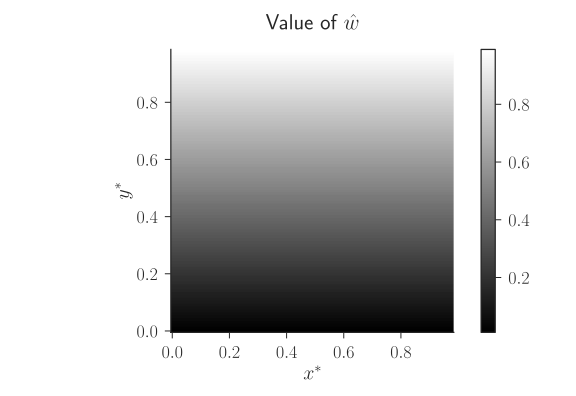
\includegraphics[width=\textwidth]{w-hat-empirical-01-marginal}
\caption{
    Estimates for $\hat{w}$ when computing $(\hat{x}, \hat{y}, \hat{w})$ using basin-hopping \citep{Wales1997} optimizing the classical marginal likelihood \eqref{eq:marginal_likelihood} (rather than a joint optimization procedure).
}
\label{fig:bl-general-marginal}
\end{figure}

\begin{figure}
\centering
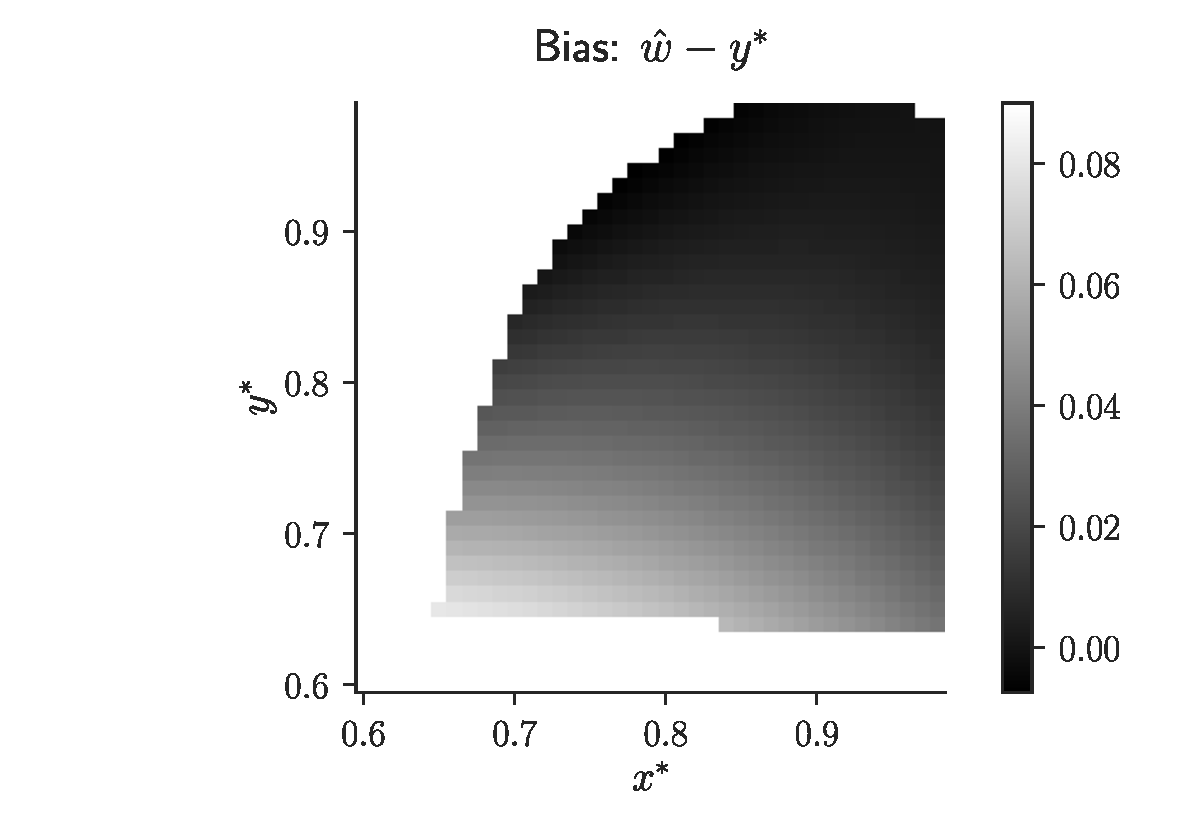
\includegraphics[width=\textwidth]{w-hat-empirical-01-bias}
\caption{
    Estimates for $\hat{w}-y^*$ when computing $(\hat{x}, \hat{y}, \hat{w})$ using basin-hopping \citep{Wales1997} optimizing \eqref{eq:profile_likelihood}.
    Plot focuses on $0.6 < x^*, y^* < 1$ where $\hat{w}$ is estimated to be a value different from 1.
    We do not compute the bias for the white region where $\hat{w}=1$ to preserve a useful scale for the rest of the plot.
}
\label{fig:bl-general-bias}
\end{figure}



\end{document}
